\documentclass{article}
\usepackage{graphicx}
\usepackage{float}
\usepackage{hyperref}
\graphicspath{ {images_latex/} }

\title{Assignment 1 Geo1001}
\author{Lisa Geers}

\begin{document}

\maketitle

\section{Introduction}
    This assignment was made for the class Geo1001. A statistical analysis was done 
    using a heat stress measurement dataset with five sensors \cite{data} . Analysing was
    done in Visual Studio Code using Python 3.7.5. Plotting was done with the use of Matplotlib.
    The source code for this assignment can be found on GitHub: \url{https://github.com/Lisageers/geo1001_hw1}
   
\section{A1}

    \subsection{Mean statistics}

        In Table 1, the calculated mean statistics of all sensors are displayed. When zoomed-in, the 
        individual values can be seen. The means of the sensors are
        quite similar for all variables. The means of the wind variables Direction - True, Wind Speed, 
        Crosswind Speed and Headwind Speed differ the most between sensors. This is logical, because 
        wind can differ greatly over short distances. This is in contrast with other variables 
        like Temperature and Relative Humidity, which are less dynamic and thus differ less in means.
        \par It stands out that the standard deviations of the variables Wind Direction True, Wind Direction Magnetic 
        and Density Altitude are higher than the other variables, meaning that there are more values 
        further from the mean. The differences in standard deviations between the sensors
        are comparable to the differences between means, differences are higher for the wind variables.
        \par The variances of Wind Direction True, Wind Direction Magnetic, Density Altitude and
        Altitude are much higher than the other variables, which means that the values of
        these variables are very spread out. The differences between sensors are, like the means and
        standard deviations, the largest for the wind-related variables.


        \begin{table}[H]
            \caption {Mean Statistics of all sensors}
            \resizebox{\columnwidth}{!}{%
            \begin{tabular}{llllllllllllllll}
            \hline
                                        & Mean A              & Mean B               & Mean C              & Mean D              & Mean E              & Standard Devation A & Standard Devation B & Standard Devation C & Standard Devation D & Standard Devation E & Variance A         & Variance B         & Variance C         & Variance D         & Variance E          \\ \hline
            Direction - True             & 209.40630048465266  & 183.41235864297255   & 183.58892481810832  & 198.32659660468877  & 223.95636363636365  & 100.54322606601899  & 99.88602389941525   & 87.76880480018731   & 90.18808156618324   & 96.47945418449655   & 10108.940307762601 & 9977.217770434554  & 7703.363096053383  & 8133.890056588521  & 9308.285079738369   \\
            Wind Speed                   & 1.290306946688207   & 1.242124394184168    & 1.3714632174616006  & 1.5816491511721908  & 0.5962424242424242  & 1.118550173932421   & 1.1408337241403745  & 1.1962107079801148  & 1.31902114073203    & 0.7150012449874839  & 1.2511544916042492 & 1.3015015861359962 & 1.4309200578862873 & 1.7398167696980256 & 0.5112267803336519  \\
            Crosswind Speed              & 0.9649434571890144  & 0.8356219709208401   & 0.9632983023443816  & 1.2105092966855295  & 0.4385050505050505  & 0.9625968857618368  & 0.9373287085891301  & 1.0210655229734091  & 1.2047833560489647  & 0.562087167714658   & 0.9265927644783866 & 0.8785851079453664 & 1.0425748022049617 & 1.4515029350126065 & 0.3159419841094861  \\
            Headwind Speed               & 0.16352988691437803 & -0.12980613893376414 & -0.2628940986257074 & -0.3005658852061439 & 0.19494949494949496 & 1.017320058054766   & 1.1210349307394734  & 1.127711035165007   & 1.1101813871607582  & 0.5648655661268653  & 1.0349401005205527 & 1.2567193159380559 & 1.2717321788329317 & 1.232502712398185  & 0.31907310779582404 \\
            Temperature                  & 17.96910339256866   & 18.065428109854604   & 17.91313662085691   & 17.99636216653193   & 18.353939393939395  & 3.9829975215127065  & 4.077875295758688   & 4.013046004830651   & 4.013177206370107   & 4.363843742775605   & 15.864269256376364 & 16.629066927759013 & 16.104538236887244 & 16.105591289728583 & 19.0431322113618    \\
            Globe Temperature            & 21.544588045234246  & 21.799434571890146   & 21.587388843977365  & 21.359296685529507  & 21.176161616161615  & 8.257805550937451   & 8.127073080259526   & 8.242651557816295   & 7.823186869859439   & 7.950817734146231   & 68.19135251709339  & 66.04931685187906  & 67.9413047035714   & 61.20225280074113  & 63.21550264161421   \\
            Wind Chill                   & 17.838206785137317  & 17.945920840064623   & 17.77299919159256   & 17.835367825383994  & 18.2940202020202    & 4.032920371452324   & 4.127447852847276   & 4.06707790227351    & 4.069011197957792   & 4.374592786175935   & 16.264446722475153 & 17.035825777973596 & 16.541122663161495 & 16.556852129105906 & 19.137062044862528  \\
            Relative Humidity            & 78.18477382875606   & 77.87831179321486    & 77.96285367825384   & 77.94203718674213   & 76.7930505050505    & 19.390978804050324  & 20.214425745479723  & 19.355170964011418  & 19.74477248514976   & 20.16170782941016   & 376.0100589791289  & 408.62300821951345 & 374.6226430461106  & 389.8560404903271  & 406.49446259849907  \\
            Heat Stress Index            & 17.899596122778675  & 18.00428109854604    & 17.82825383993533   & 17.92162489894907   & 18.286424242424246  & 3.8725764449092246  & 3.929269324233937   & 3.9187055976553324  & 3.88814143003908    & 4.2982833827256695  & 14.99684832166577  & 15.439157422365822 & 15.356253561095237 & 15.117643779986343 & 18.475240038215624  \\
            Dew Point                    & 13.553877221324719  & 13.530856219709205   & 13.458124494745352  & 13.50860953920776   & 13.558787878787879  & 3.118248198871891   & 3.1042741850691207  & 3.17555498985501    & 3.1736230057997945  & 3.069623011701569   & 9.723471829767792  & 9.636518216086554  & 10.084149493593053 & 10.071882982941721 & 9.42258543396781    \\
            Psychro Wet Bulb Temperature & 15.270718901453955  & 15.295516962843294   & 15.196645109135003  & 15.26018593371059   & 15.406666666666666  & 2.63515220041187    & 2.6019728519991188  & 2.690597228681732   & 2.6541294009257097  & 2.645268499131606   & 6.944027119335519  & 6.770262722540429  & 7.239313446989817  & 7.044402876858267  & 6.997445432497979   \\
            Station Pressure             & 1016.1682552504037  & 1016.6570274636512   & 1016.689329021827   & 1016.7280113177042  & 1016.1661010101009  & 6.202520988371144   & 6.069755714457117   & 6.139339656821912   & 5.915047217819551   & 6.240185369824895   & 38.47126661118455  & 36.841934433184825 & 37.69149142182619  & 34.98778358903481  & 38.93991344977666   \\
            Barometric Pressure          & 1016.1284329563813  & 1016.6164781906298   & 1016.6518997574777  & 1016.6888843977364  & 1016.127797979798   & 6.202253690096152   & 6.068679242921268   & 6.1380471779360235  & 5.912049294318023   & 6.239805833414894   & 38.467950836311324 & 36.82886775346346  & 37.67562315856838  & 34.952326858446234 & 38.93517683871854   \\
            Altitude                     & -25.98707592891761  & -30.05815831987076   & -30.338722716248988 & -30.653193209377527 & -25.96121212121212  & 51.6104741793961    & 50.45501096417206   & 51.07381554372864   & 49.19068601563611   & 51.88789247750703   & 2663.6410450221115 & 2545.708131394723  & 2608.5346341948175 & 2419.723590688898  & 2692.3533857573307  \\
            Density Altitude             & 137.31663974151857  & 135.58077544426493   & 129.62287793047696  & 132.41107518189168  & 150.84              & 162.8190539993073   & 163.90030579705498  & 164.2759963297163   & 162.83772822207789  & 172.380183031638    & 26510.04434522935  & 26863.310240368137 & 26986.602970120963 & 26516.1257325273   & 29714.92750202102   \\
            NA Wet Bulb Temperature      & 15.981542810985461  & 15.996809369951535   & 15.934236054971707  & 15.915642683912694  & 15.93688888888889   & 3.164191473248514   & 3.1319729344666056  & 3.2373259175903097  & 3.1602901986945207  & 3.071186013000985   & 10.0121076793786   & 9.80925446223136   & 10.48027909670194  & 9.987434139964652  & 9.432183526452889   \\
            WBGT                         & 17.25432148626817   & 17.321970920840062   & 17.22502021018593   & 17.1767987065481    & 17.185535353535354  & 4.01687167891727    & 3.979366214290523   & 4.067769087518241   & 3.937916313886086   & 3.935717409847468   & 16.13525808488765  & 15.835355467436887 & 16.546745349368983 & 15.50718489517018  & 15.489871530176462  \\
            TWL                          & 301.39293214862676  & 299.45169628432956   & 301.8997574777688   & 305.254567502021    & 284.11531313131314  & 28.54411610414145   & 28.108170010939546  & 27.68634164875935   & 24.819544864349226  & 35.915364164052534  & 814.7665641667074  & 790.0692213638812  & 766.5335138918265  & 616.009807273444   & 1289.913383036509   \\
            Direction - Mag              & 208.90508885298868  & 183.2172859450727    & 183.08367016976555  & 197.8261924009701   & 223.89656565656566  & 100.52699661703112  & 99.87715909634285   & 87.77596578759673   & 90.19598390521257   & 96.27049335275693   & 10105.677048840585 & 9975.446909156182  & 7704.620169945353  & 8135.315512629364  & 9268.007890383216   \\ \hline
            \end{tabular}
        }
            \end{table}


    \subsection{Histograms}
        \begin{figure}[H]
            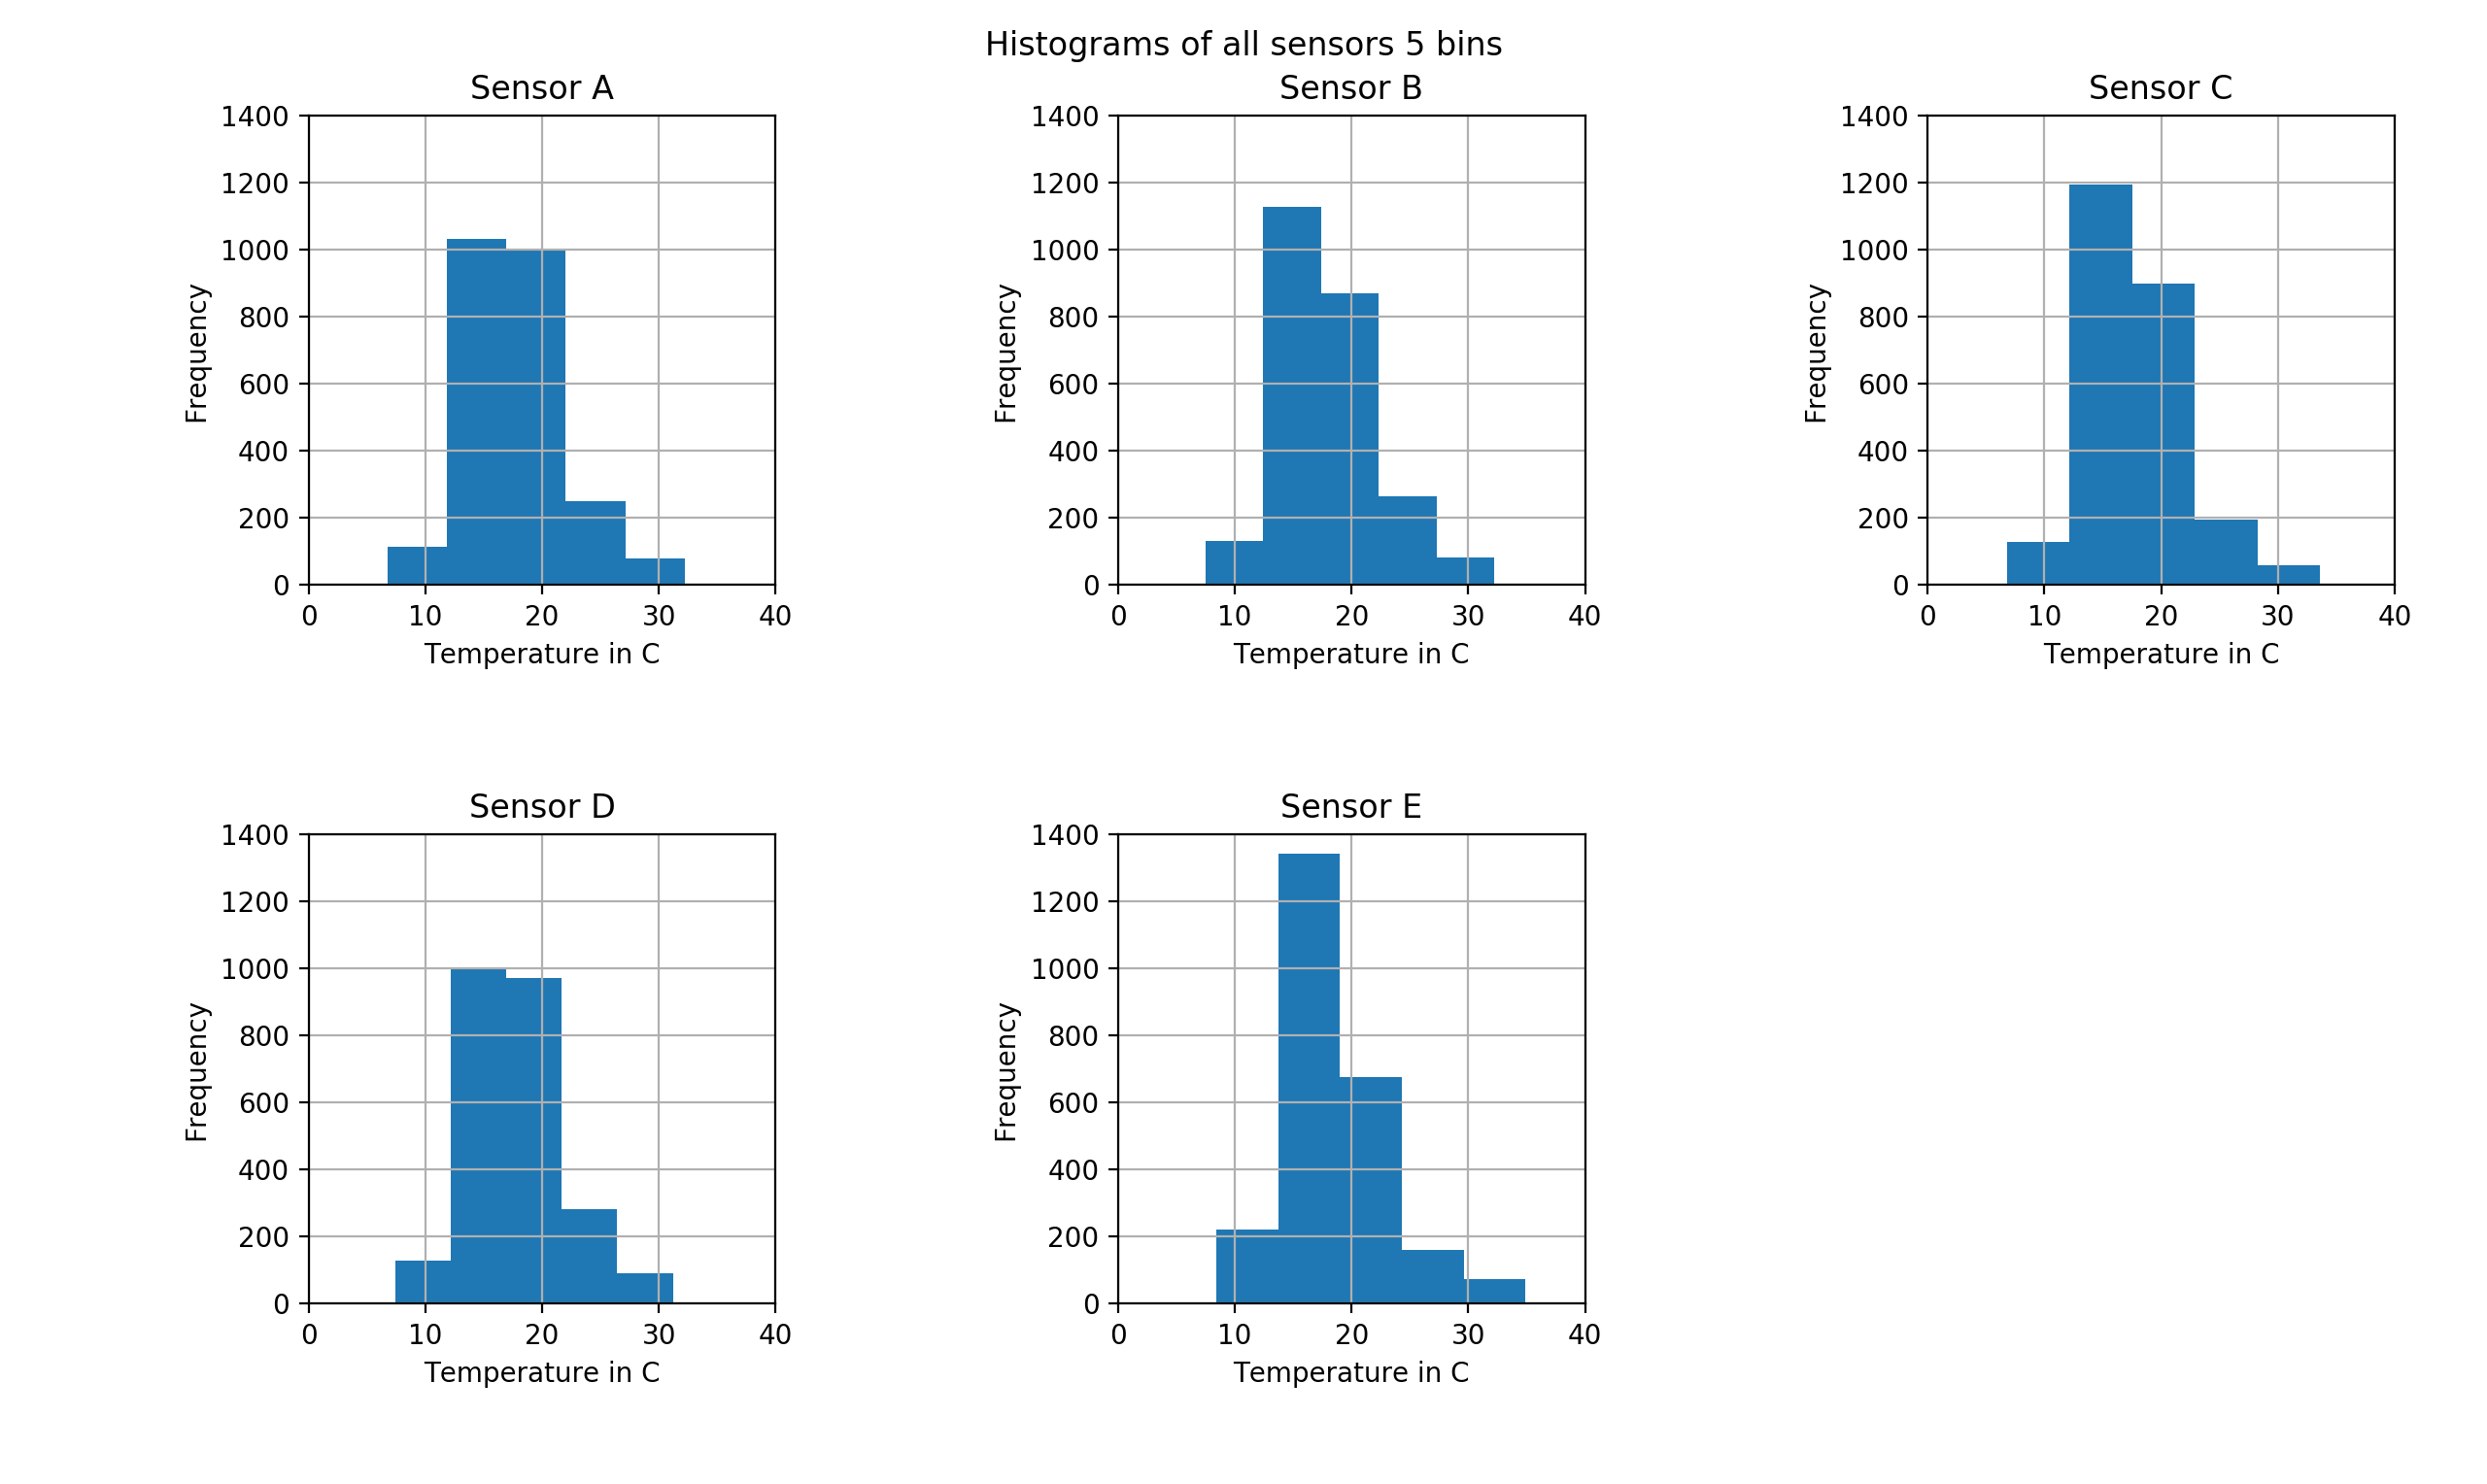
\includegraphics[width=\textwidth]{histogram_5_bins}
            \caption{Histograms of all sensors with 5 bins}
        \end{figure}

        \begin{figure}[H]
            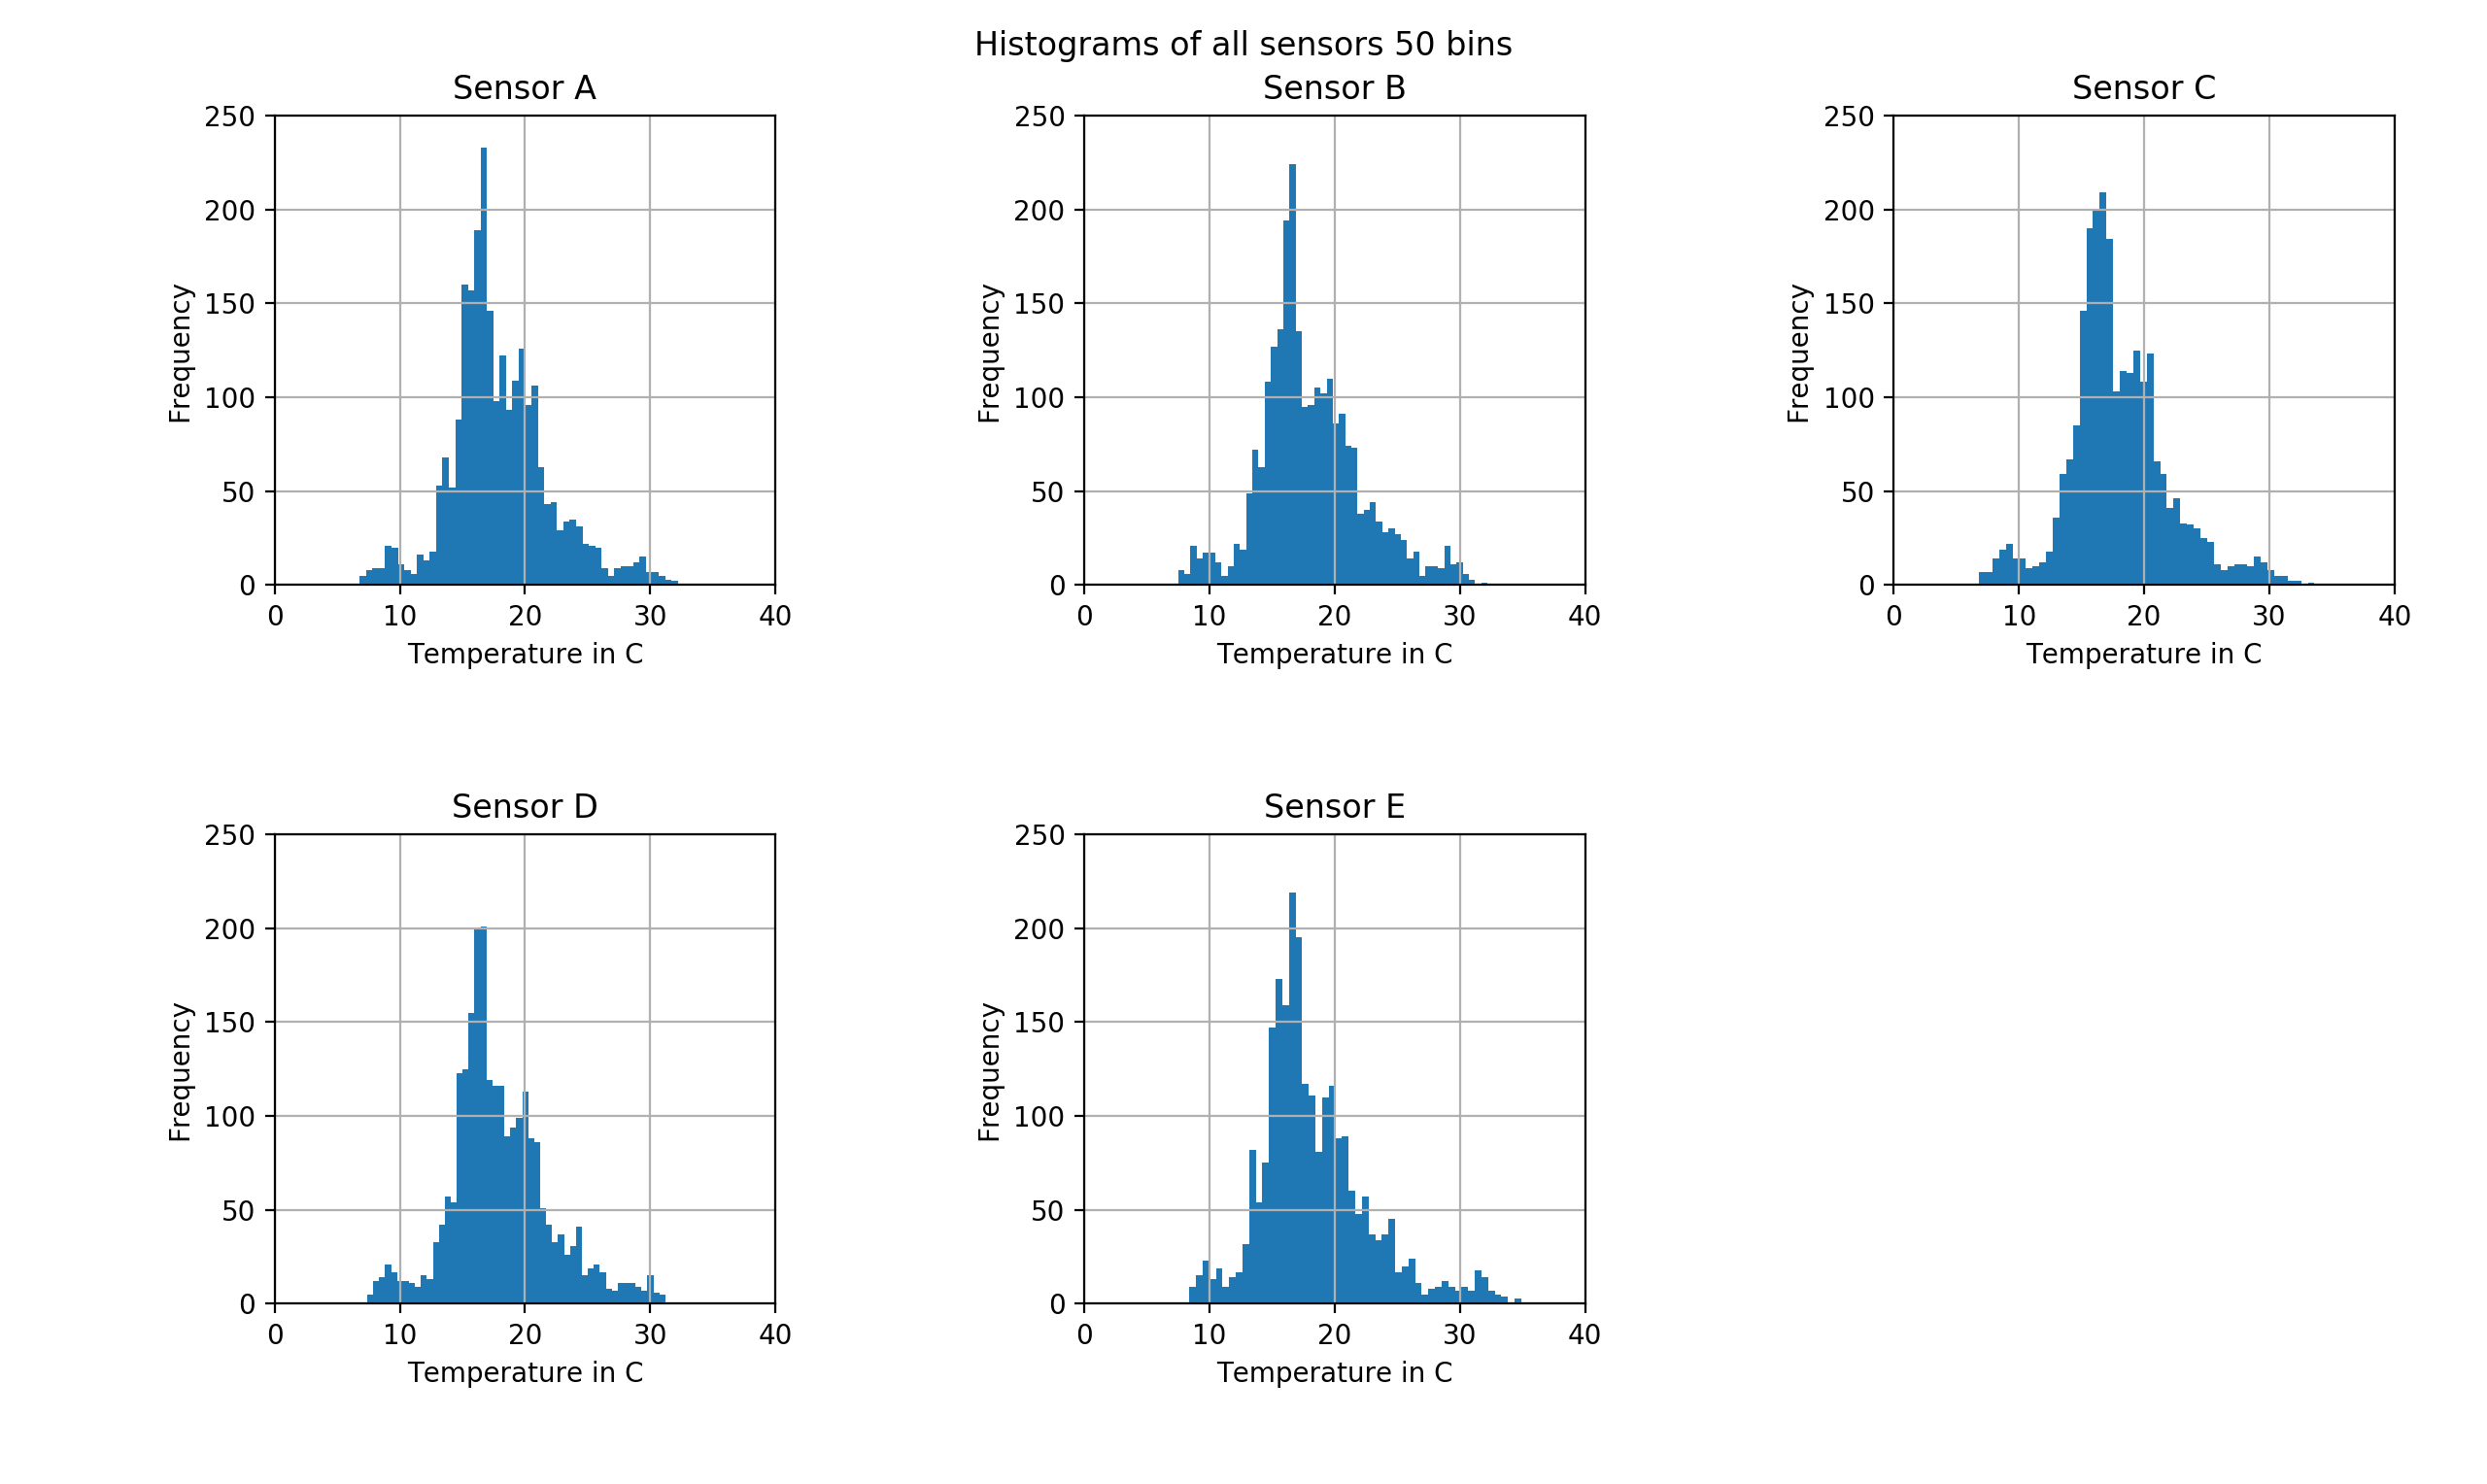
\includegraphics[width=\textwidth]{histogram_50_bins}
            \caption{Histograms of all sensors with 50 bins}
        \end{figure}
        
        In Figures 1 and 2, the five histograms of the Temperature variable are displayed.
        As can be seen, there is a significant difference between the figures due to the bin sizes.
        Figure 2 with binsize 50 is much more detailed, which makes this figure more useful for analysation.
        This shows that the number of bins is important in order to be able to do the right analysation.
        The binsize calculated with Rice's rule is approximately in the middle between 5 and 50. 
        Rice's rule \ 2 * $\sqrt[3]{N}$ \ with \ N = 2474 \ gives 27 as a number of bins. 



    \subsection{Frequency polygons}
        \begin{figure}[H]
            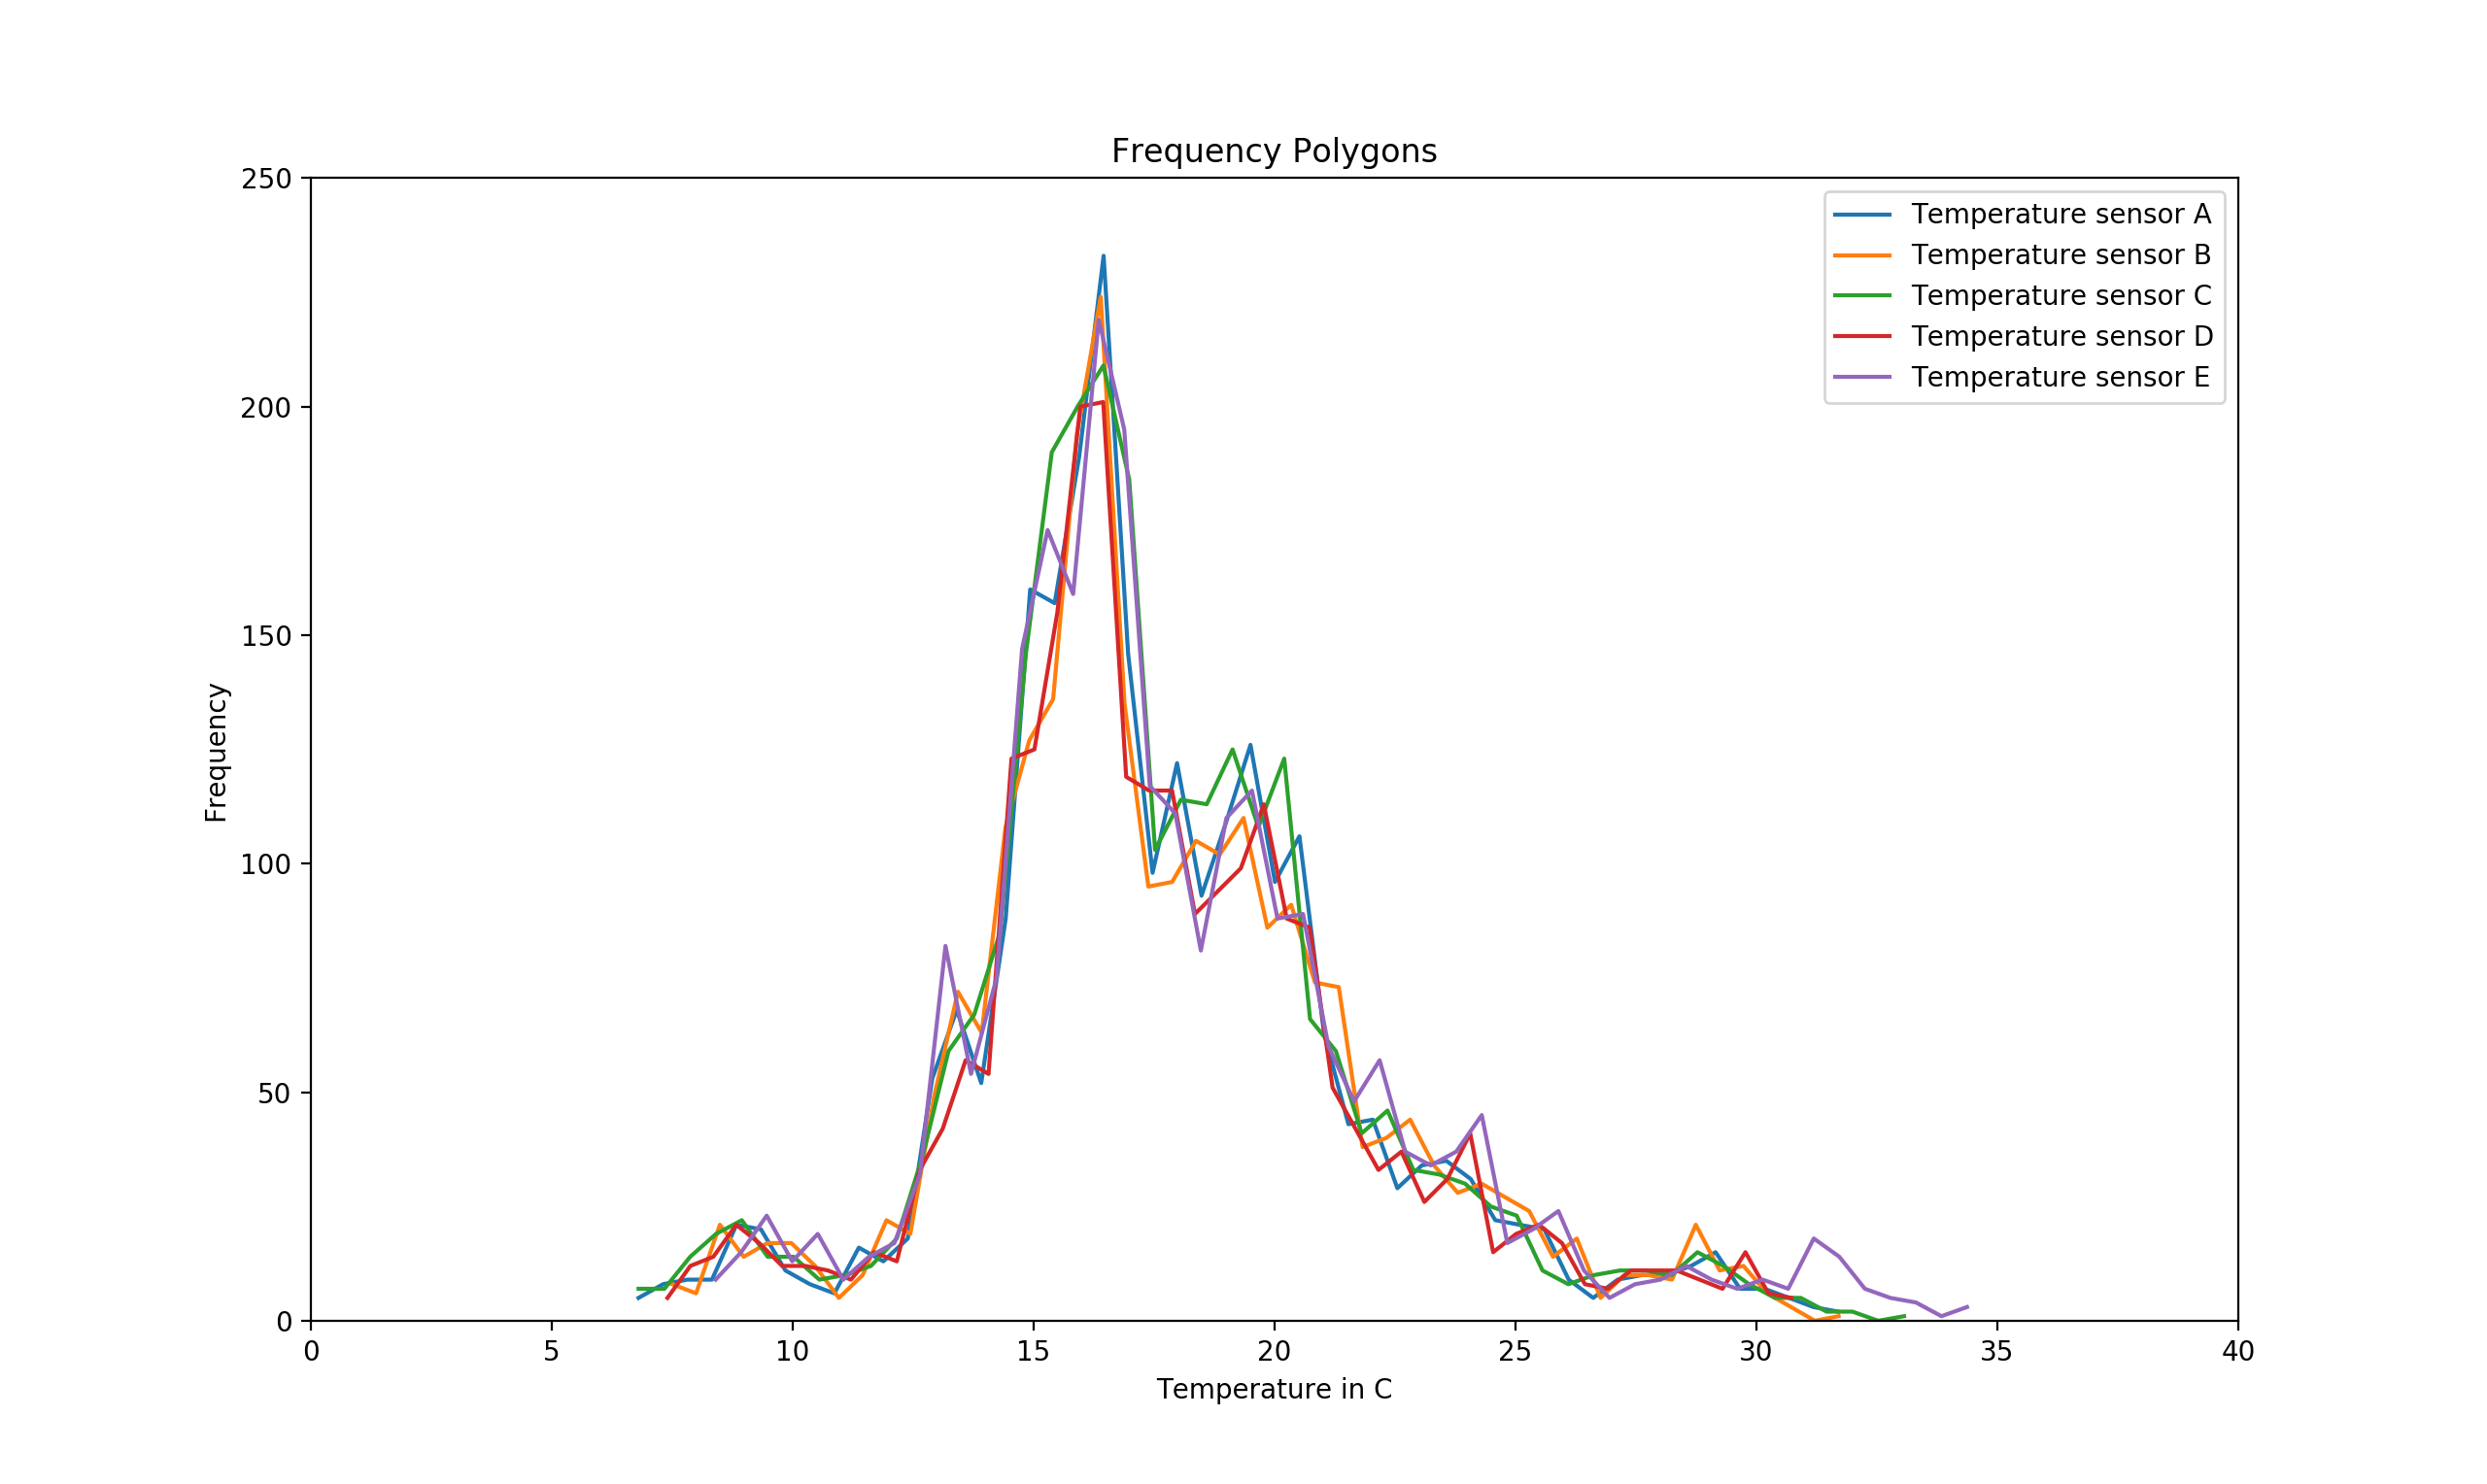
\includegraphics[width=\textwidth]{frequency_polygons_temp}
            \caption{Frequency polygon of all sensors for the variable Temperature}
        \end{figure}
            

    \subsection{Boxplots}
        
        \begin{figure}[H]
            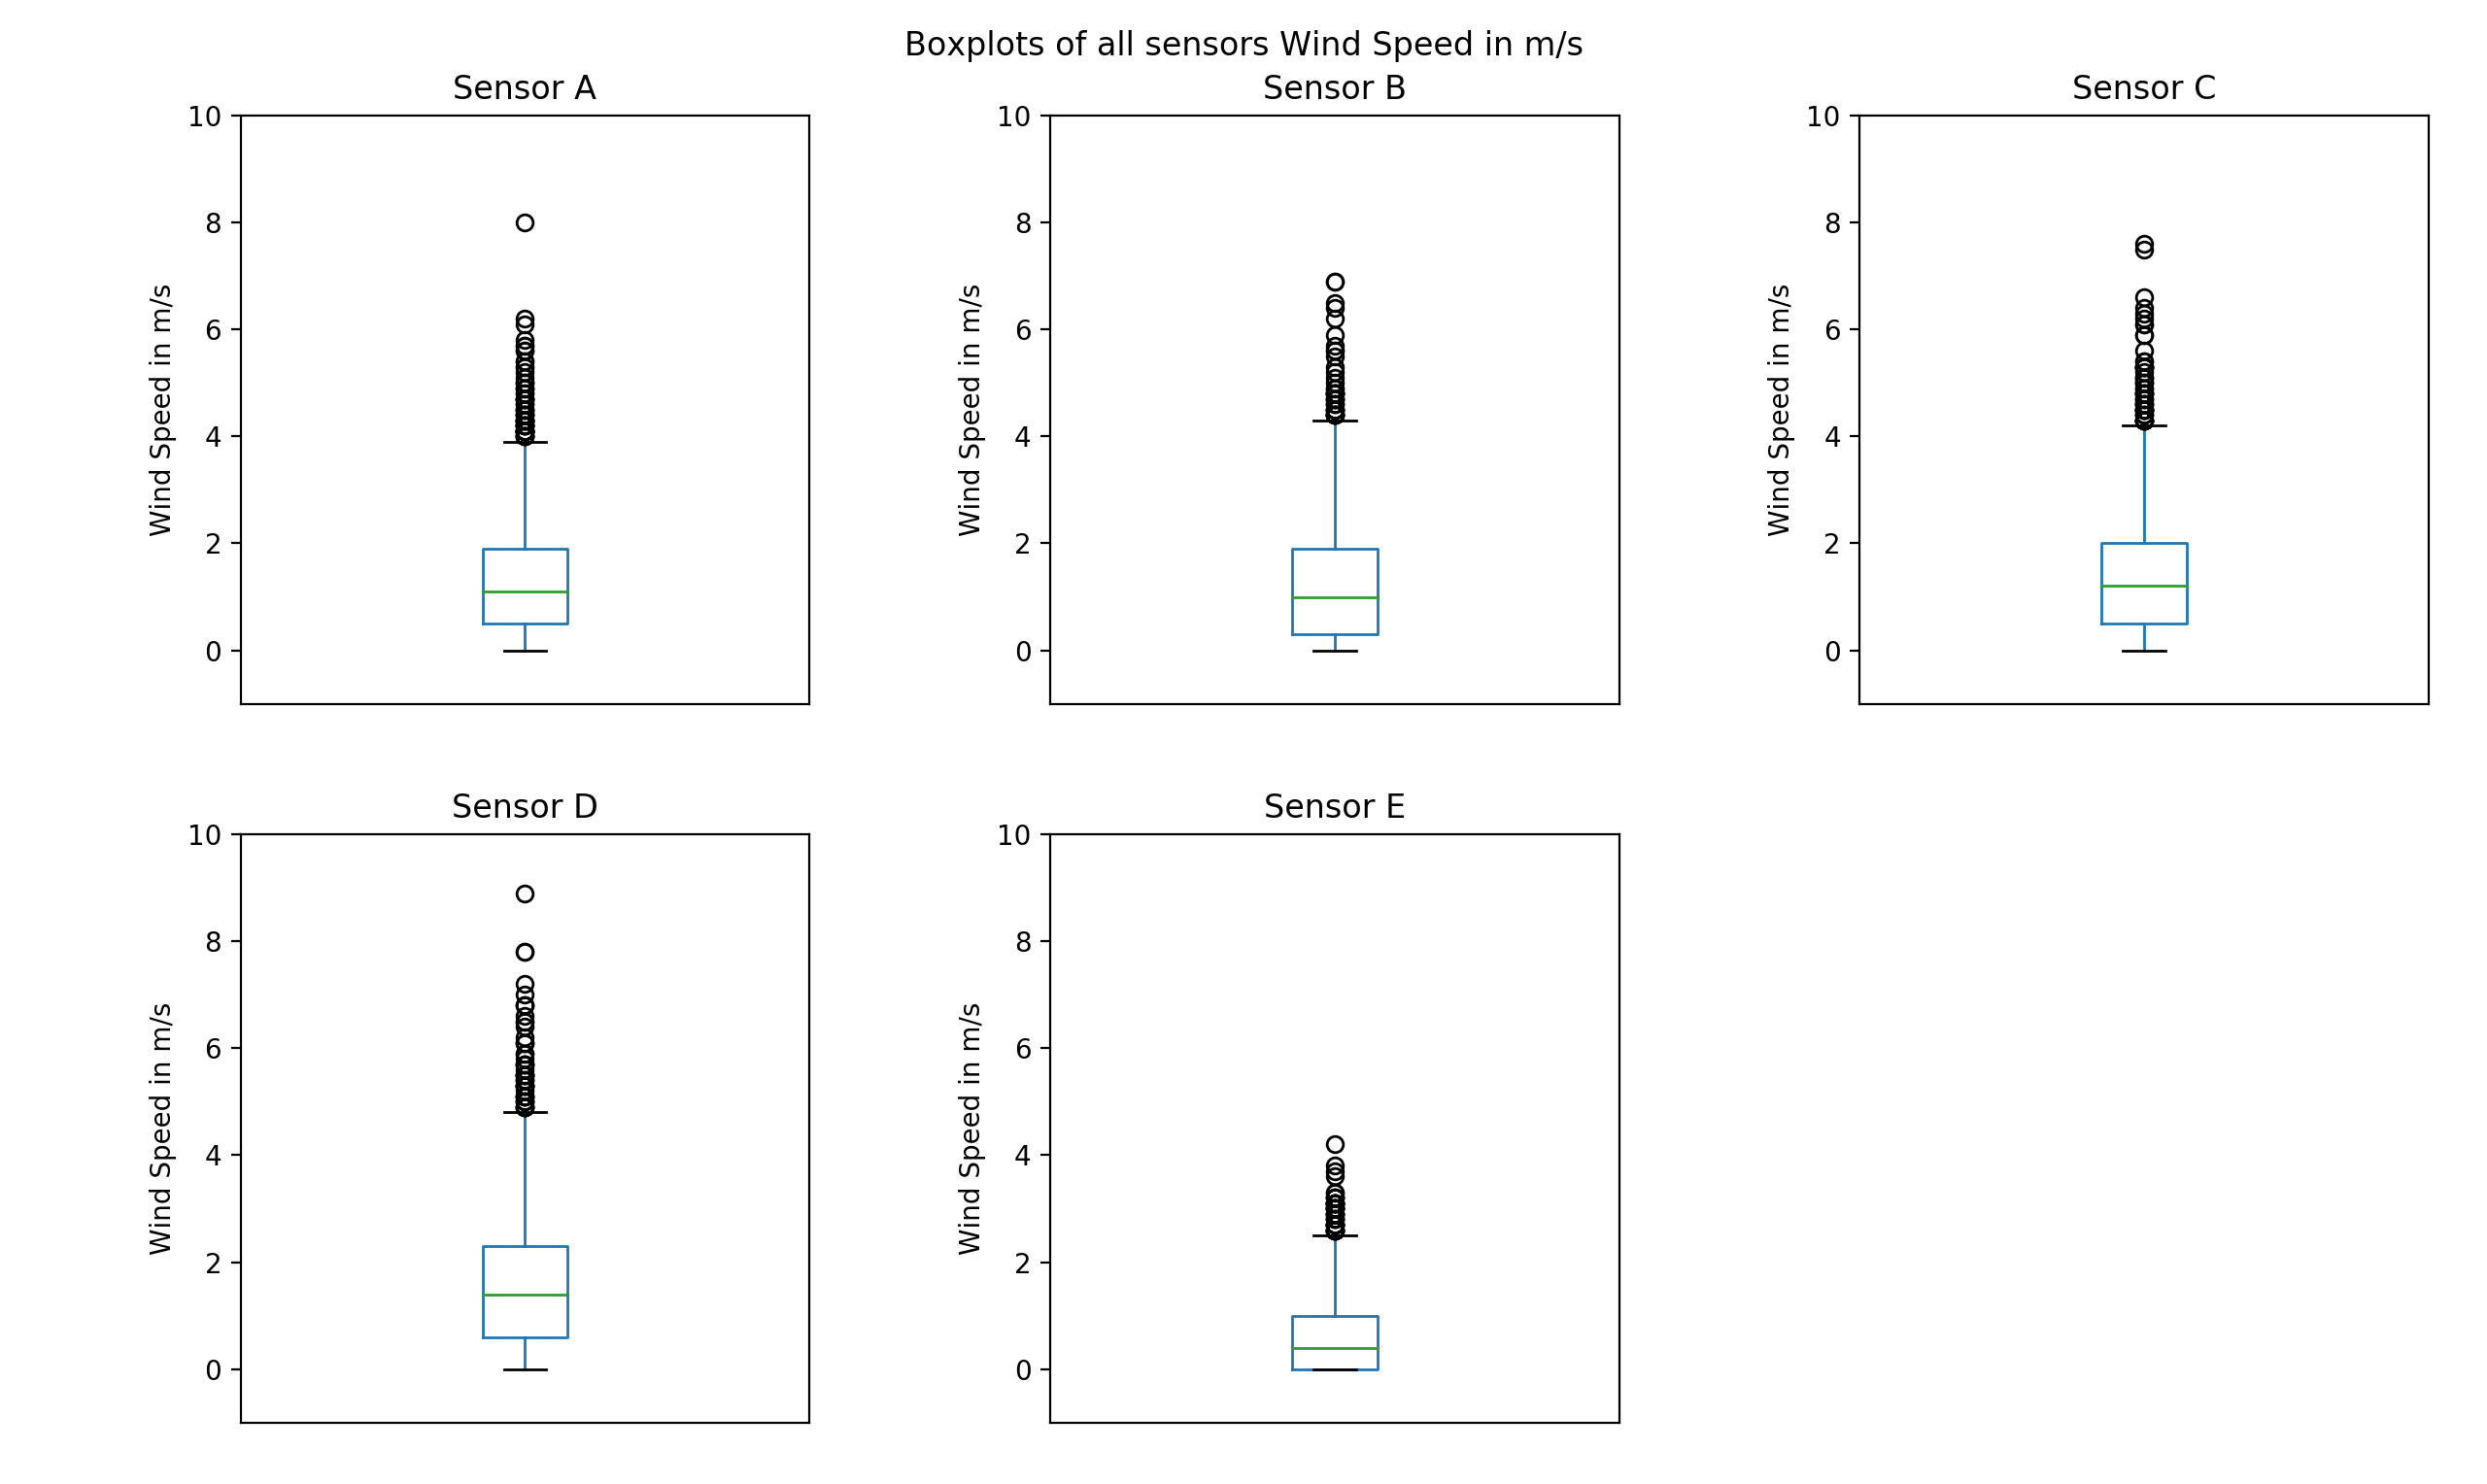
\includegraphics[width=\textwidth]{boxplot_windspeed}
            \caption{Boxplots of all sensors for the variable Wind Speed}
        \end{figure}
        
        \begin{figure}[H]
            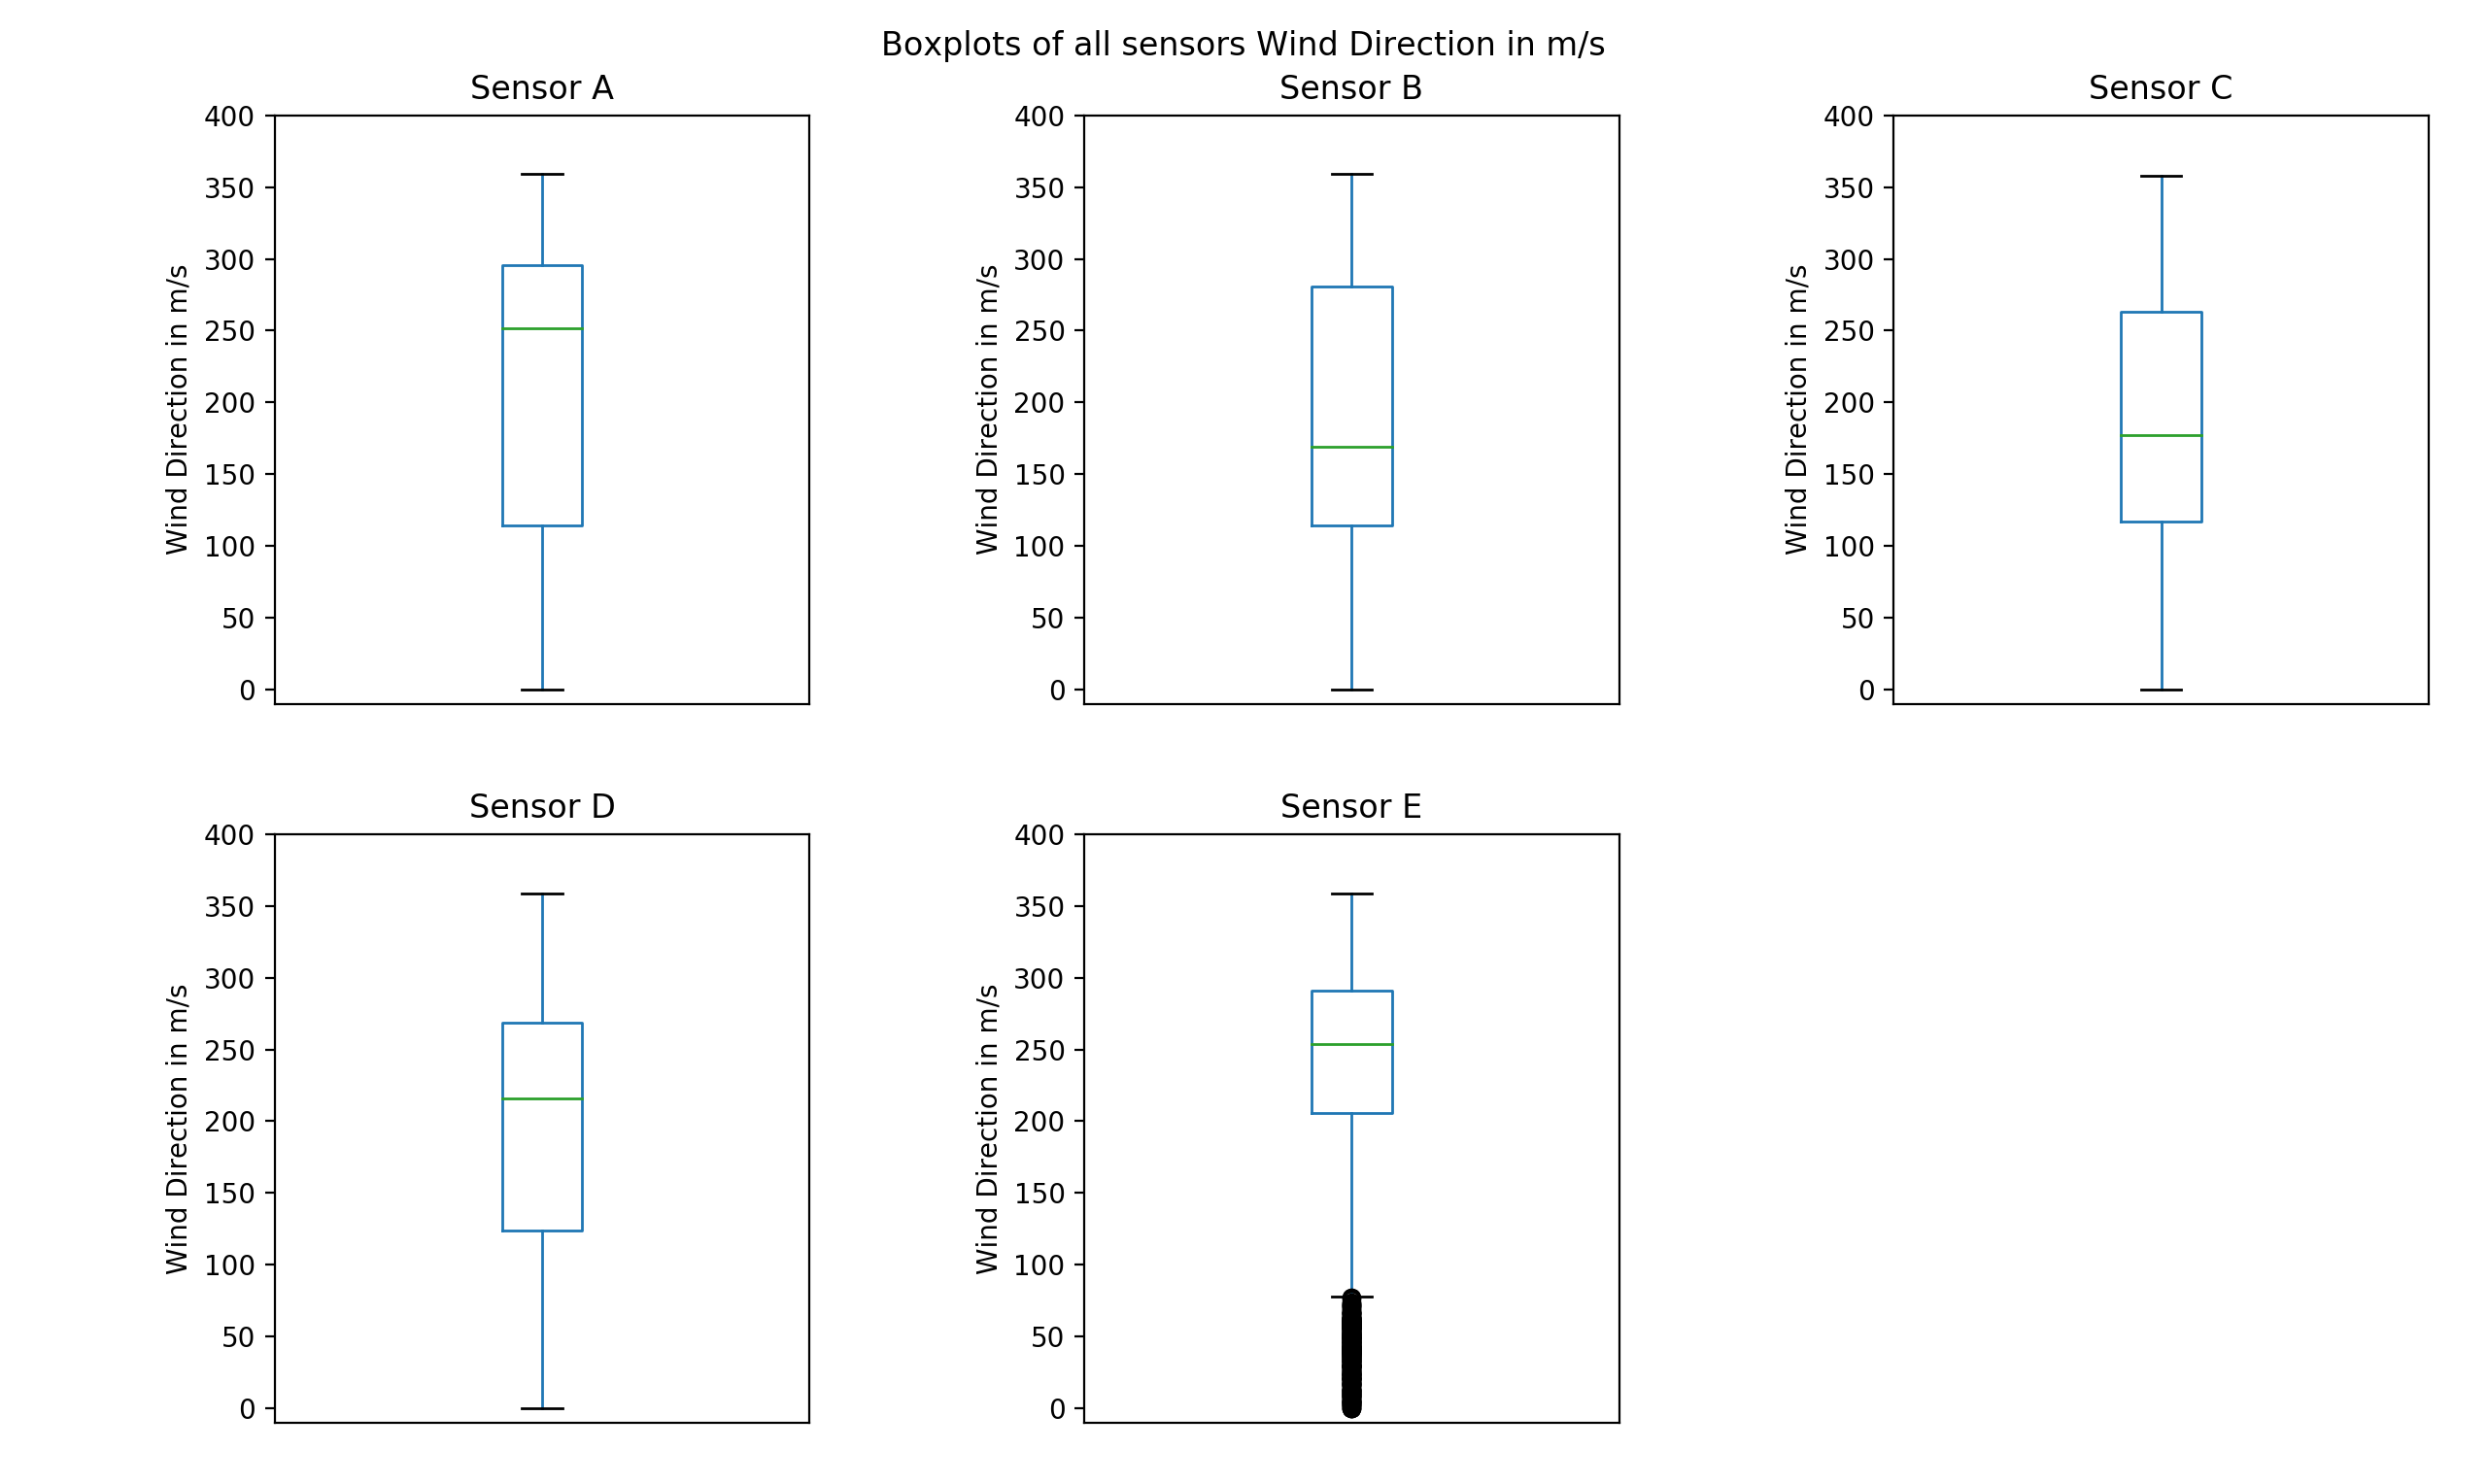
\includegraphics[width=\textwidth]{boxplot_winddirection}
            \caption{Boxplots of all sensors for the variable Wind Direction}
        \end{figure}
        
        \begin{figure}[H]
            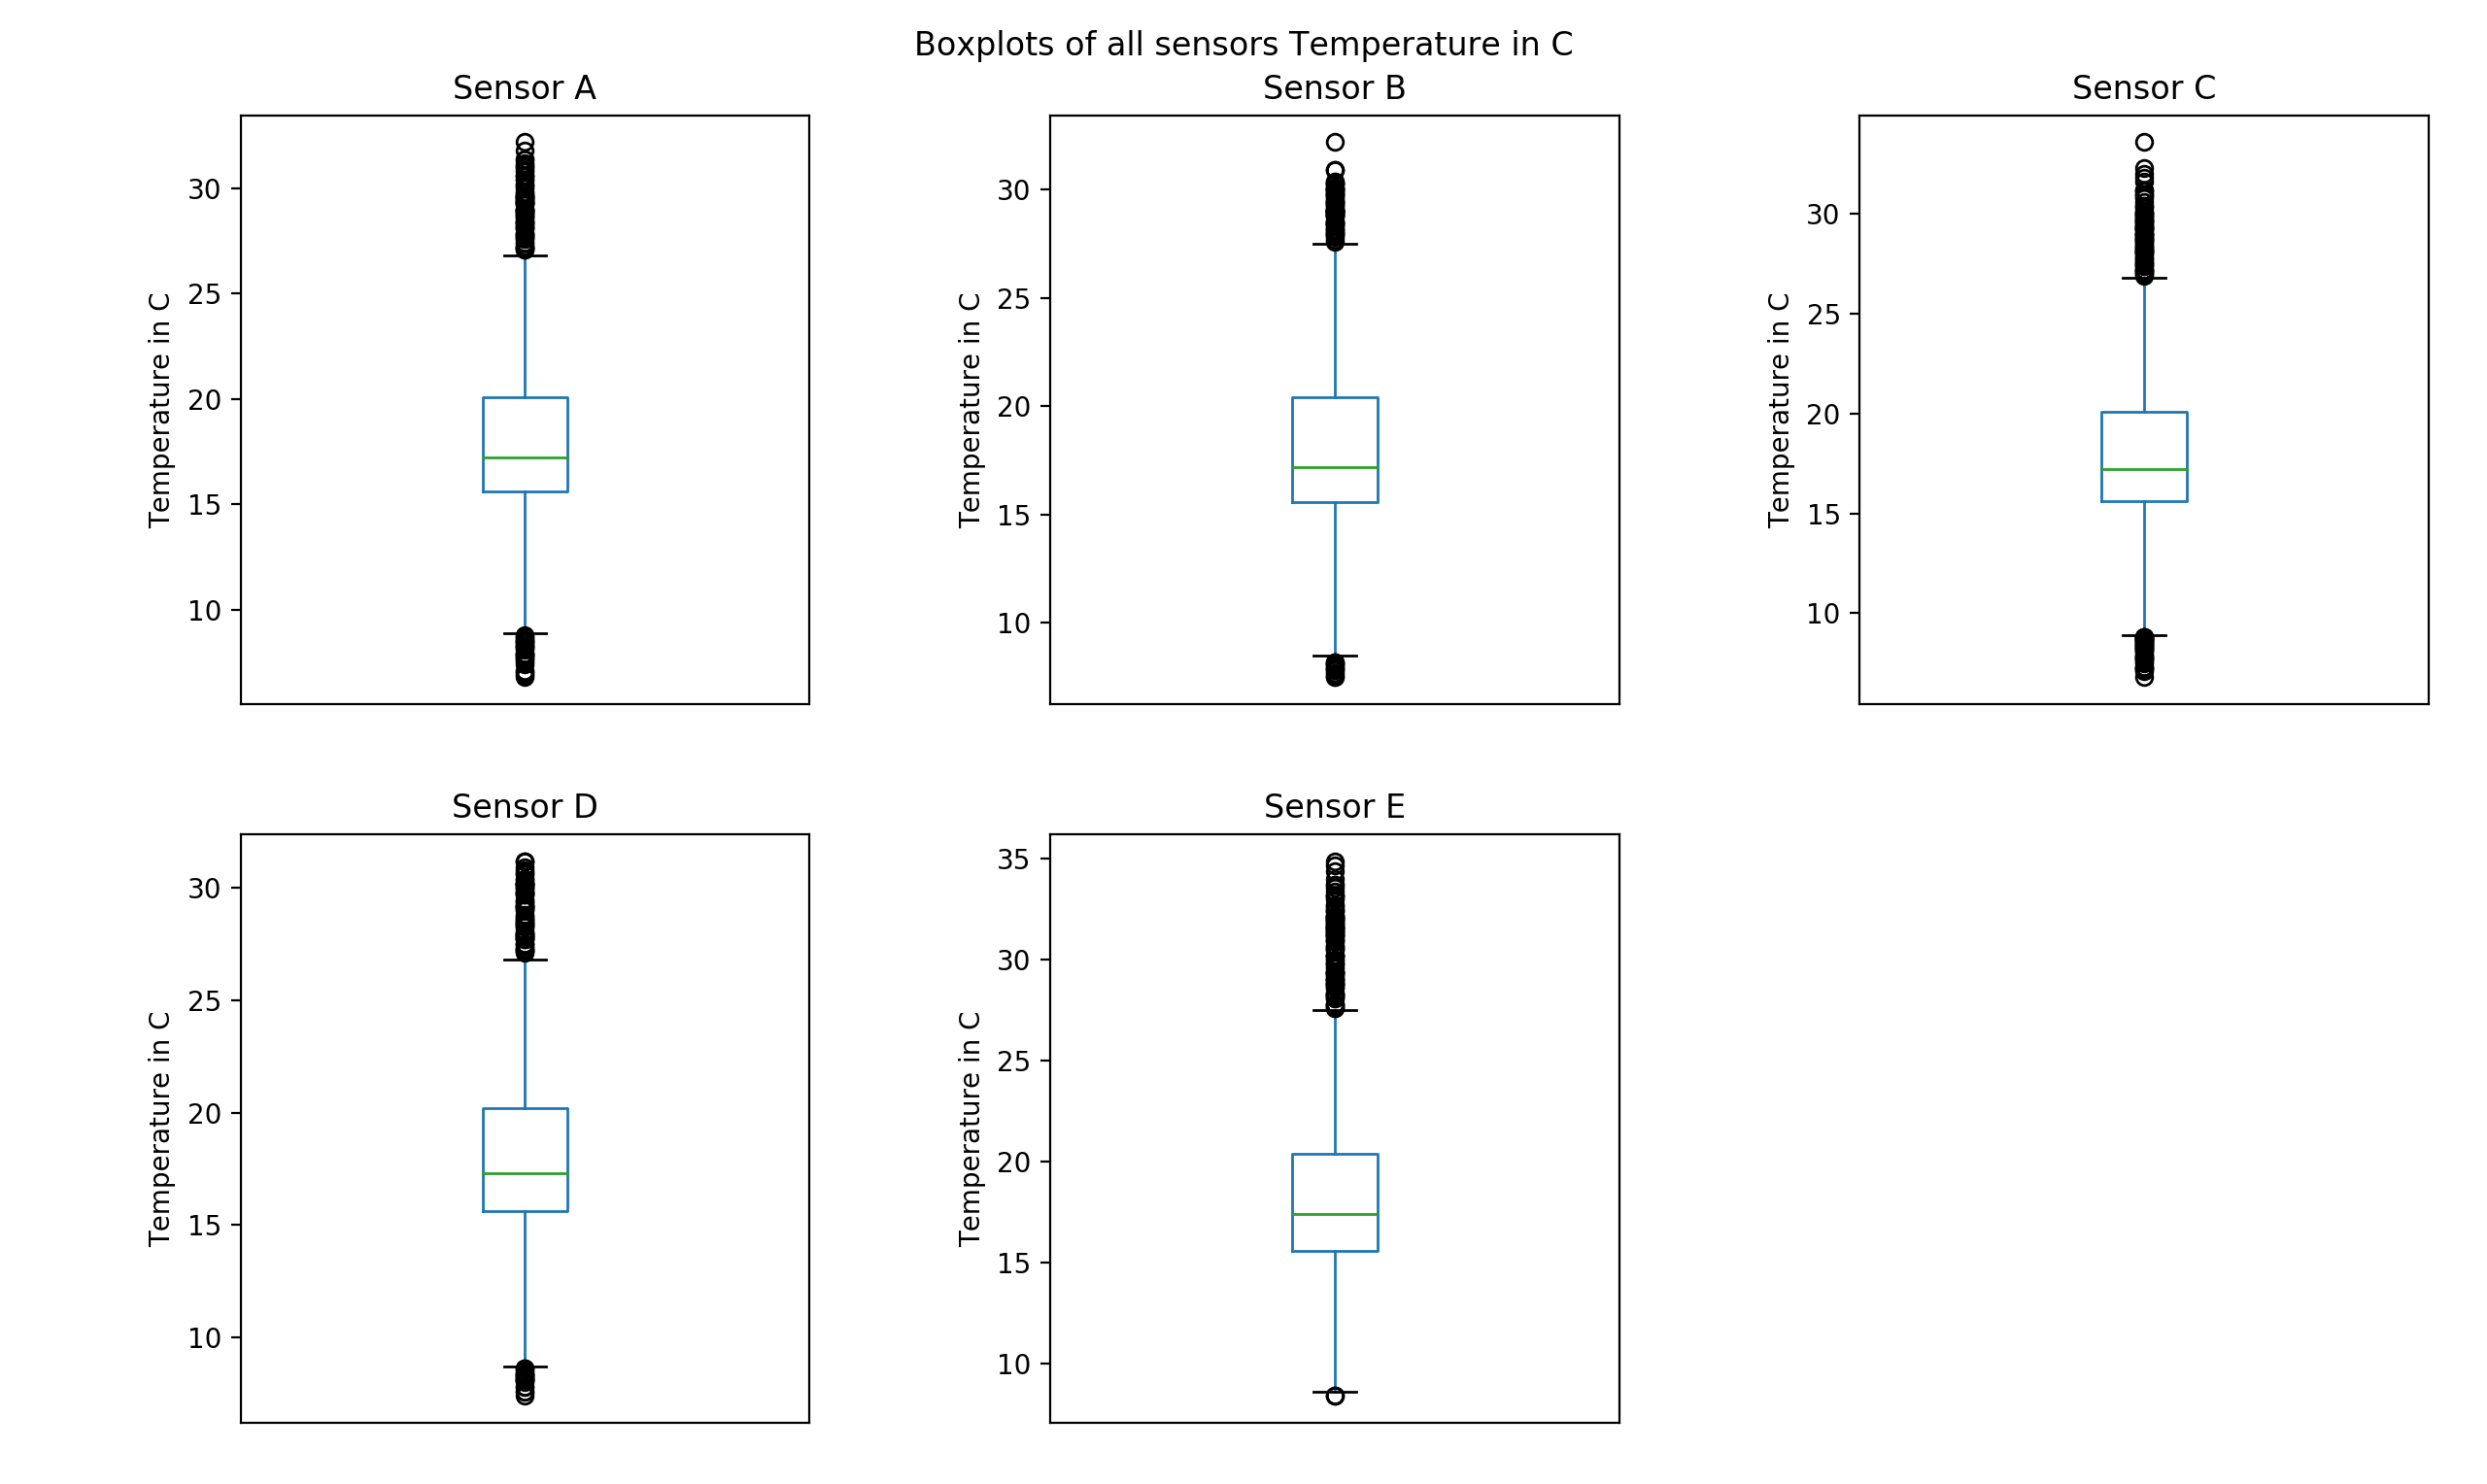
\includegraphics[width=\textwidth]{boxplot_temperature}
            \caption{Boxplots of all sensors for the variable Temperature}
        \end{figure}
        

\section{A2}
        \subsection{Functions Temperature}
            \begin{figure}[H]
                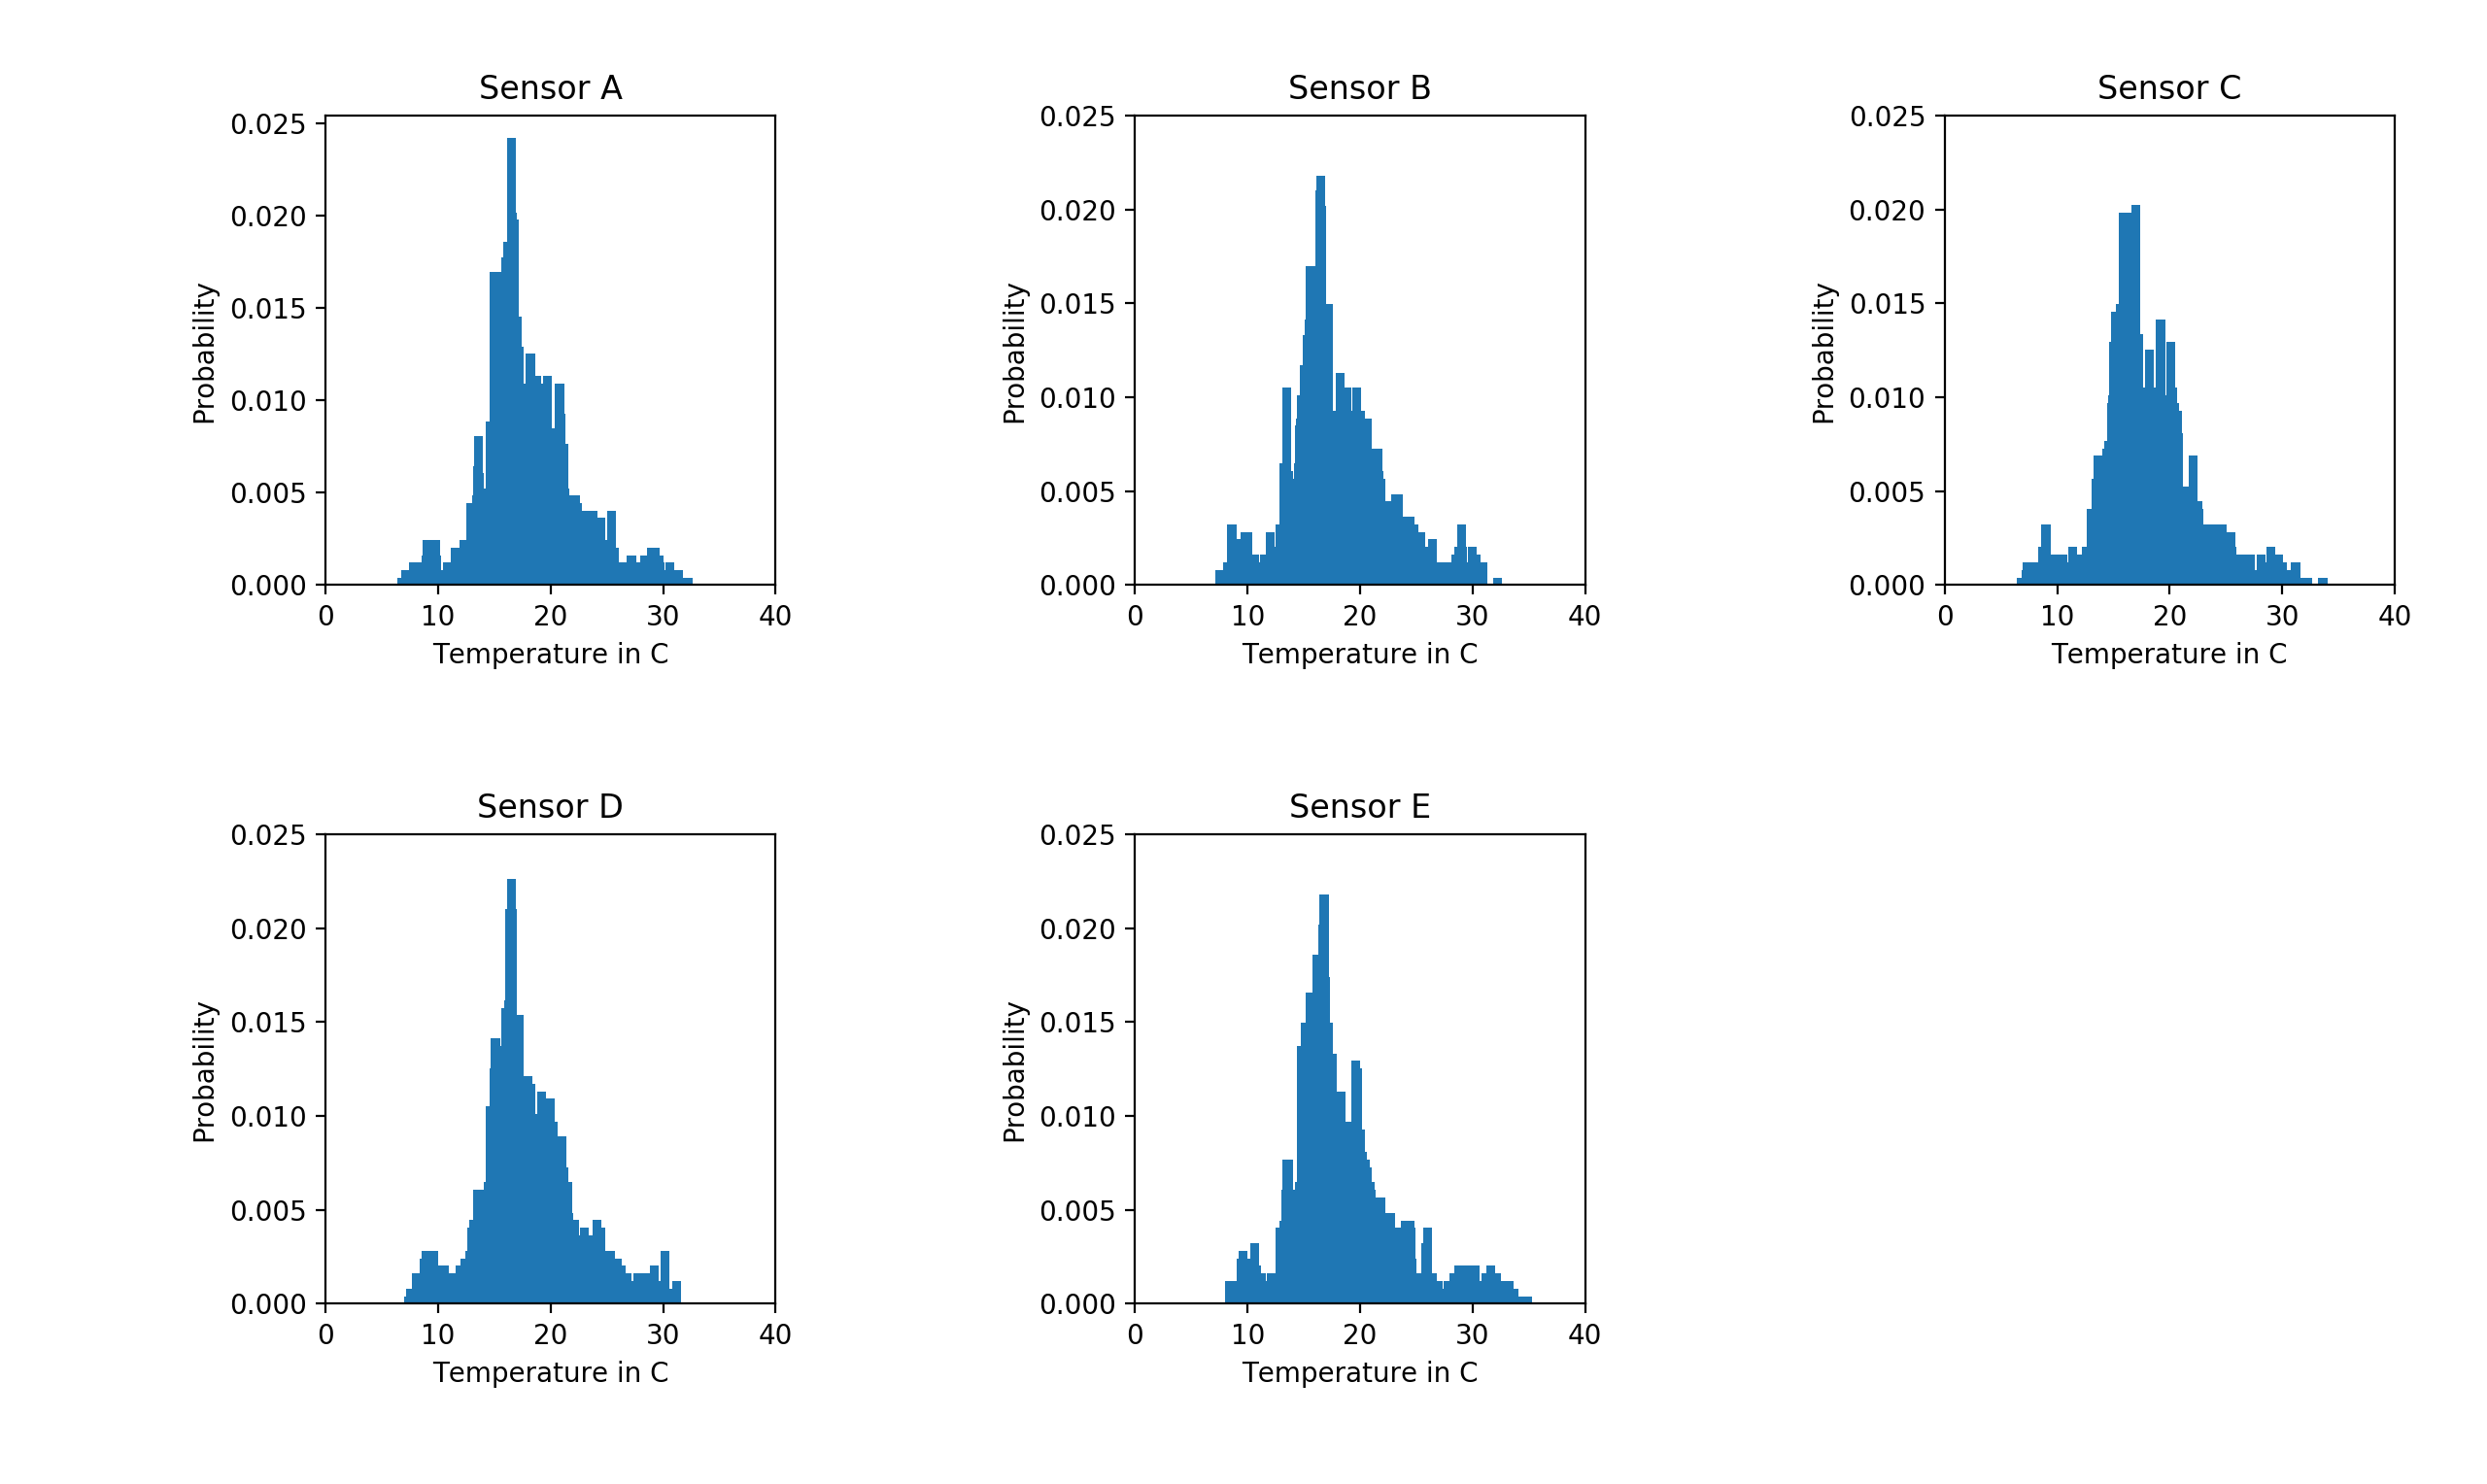
\includegraphics[width=\textwidth]{pmf_temp}
                \caption{Probability Mass Functions of Temperature for all sensors}
            \end{figure}

            The probability mass functions (Figure 7) of the different sensors look similar and are relatively normal
            distributed. The left side of the curves look steeper, meaning that the
            distributions are slightly skewed positively. Sensor E is skewed the most compared
            to the other sensors.

            \begin{figure}[H]
                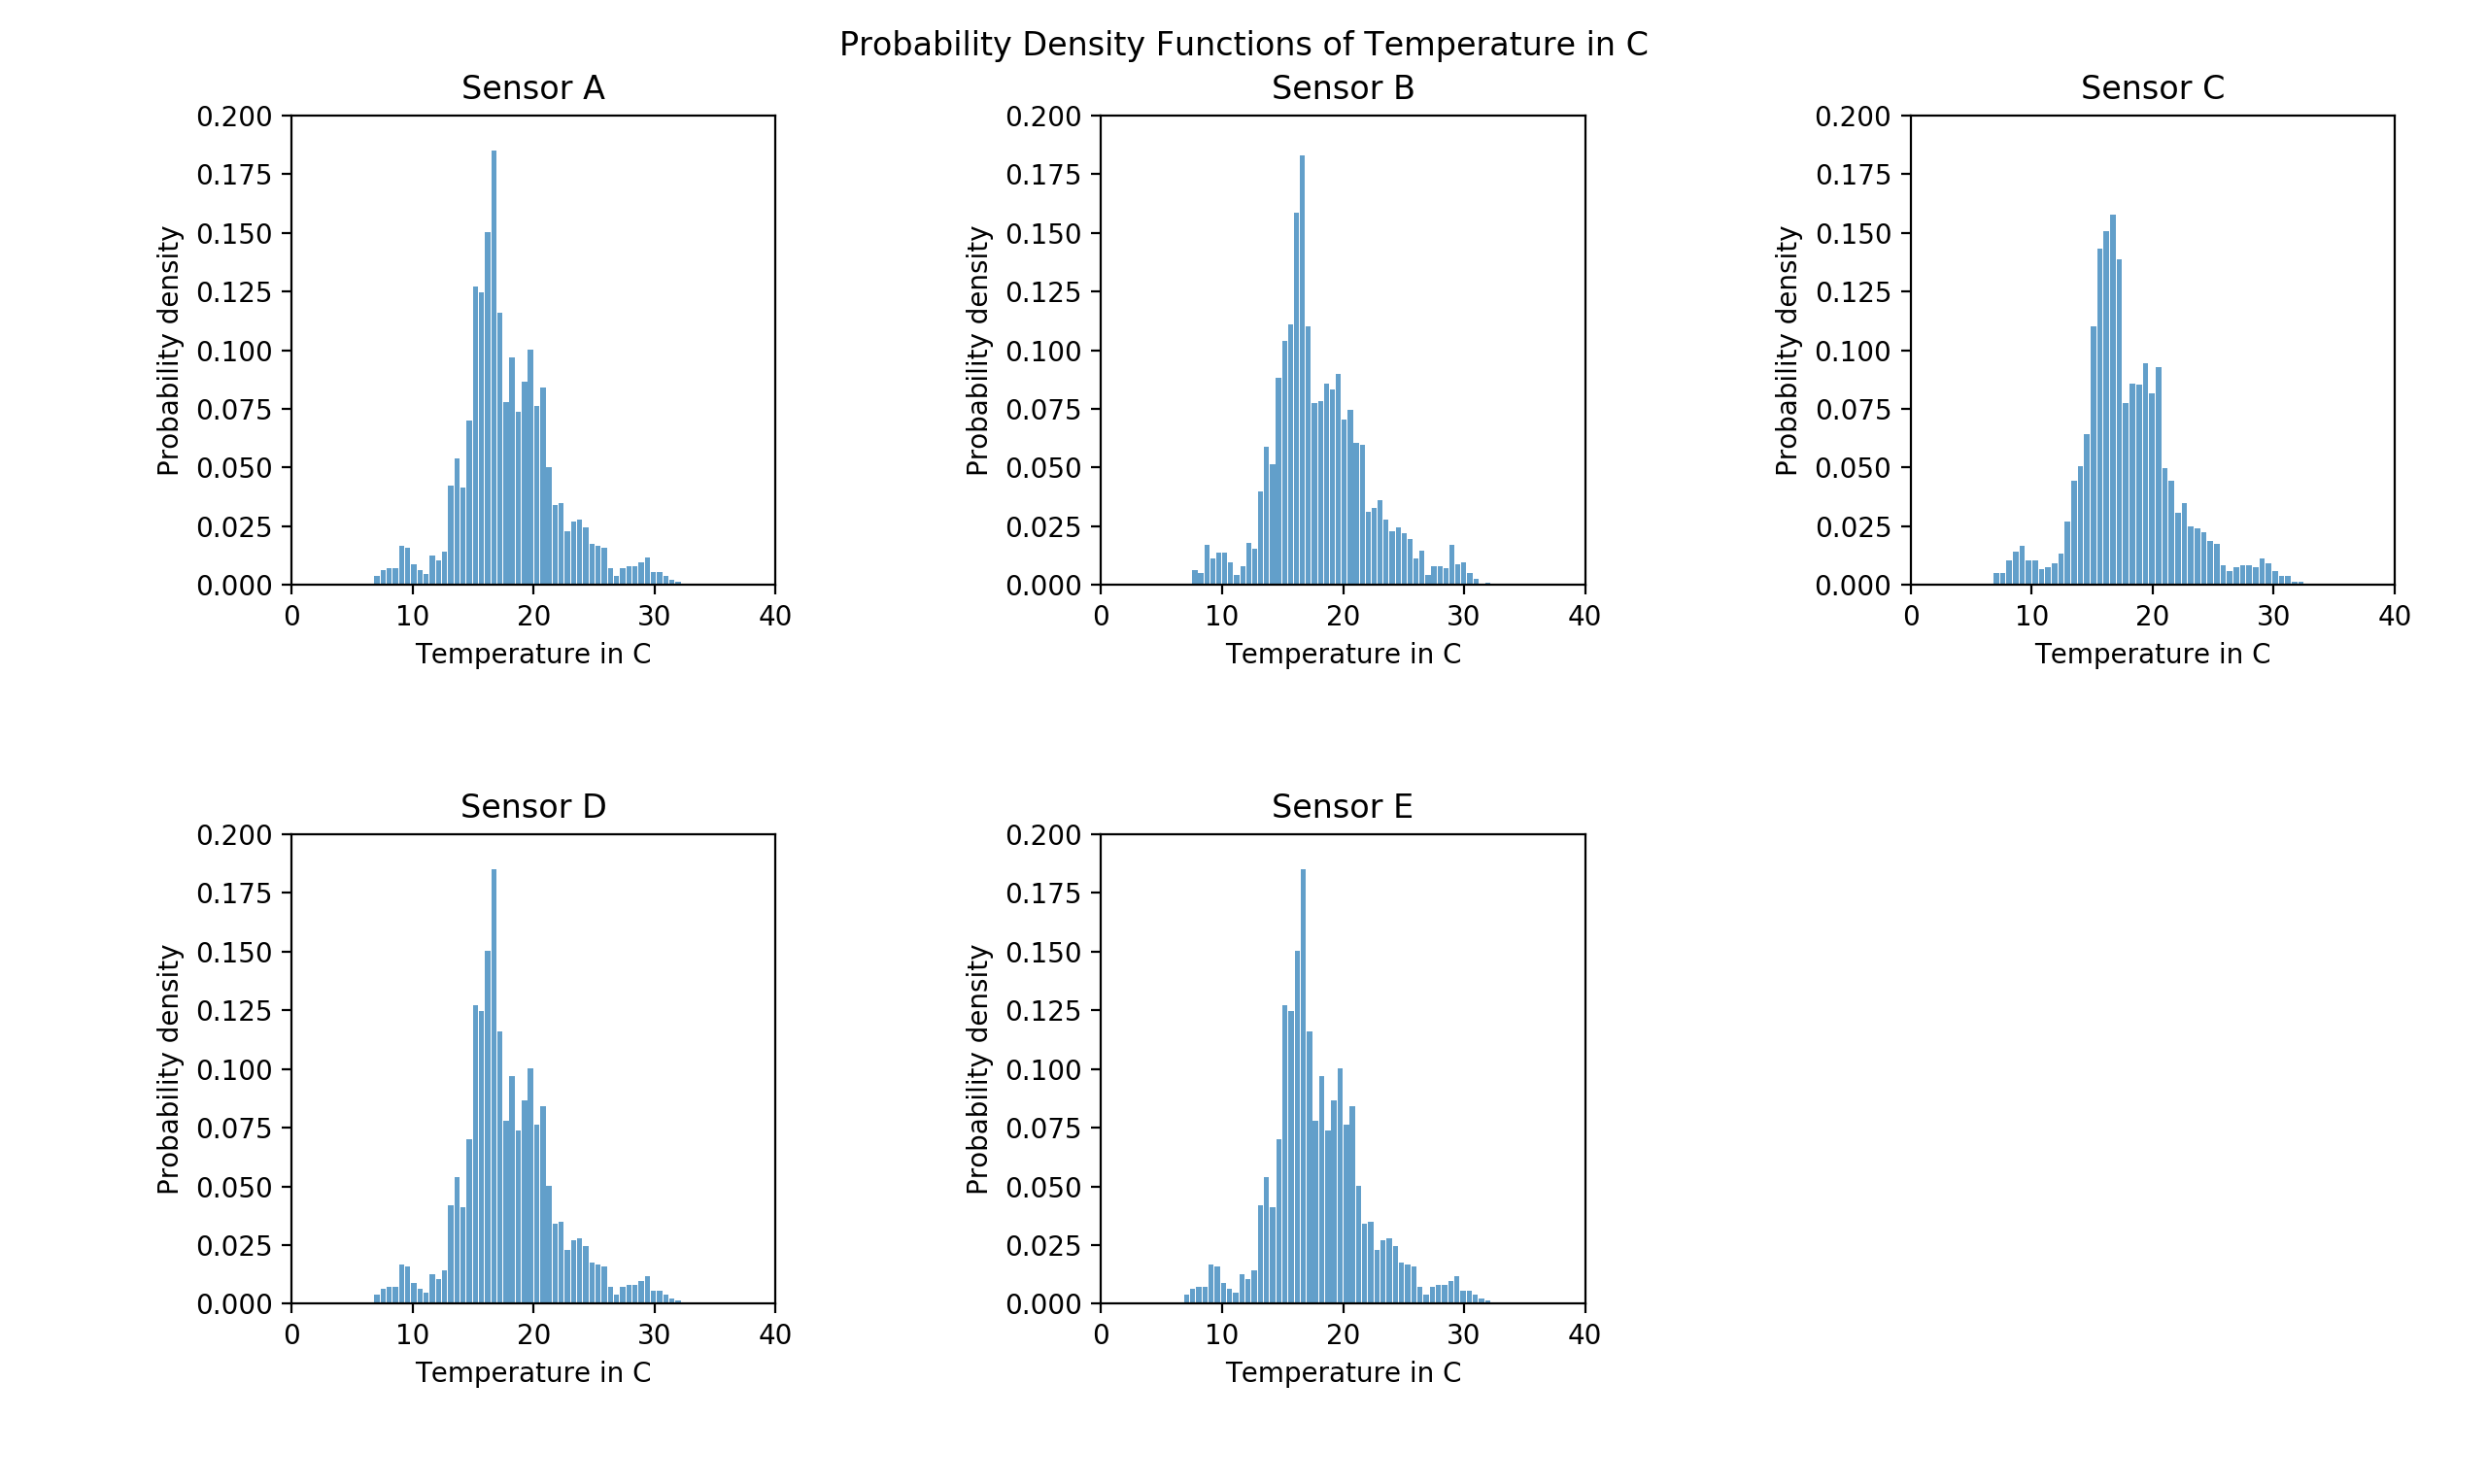
\includegraphics[width=\textwidth]{pdf_temp}
                \caption{Probability Density Functions of Temperature for all sensors}
            \end{figure}

            The behaviours of the probability density functions (Figure 8) are similar to the 
            probability mass functions. They are slightly positively skewed. In these plots the 
            bimodal properties of the data can be seen more clearly. All plots show two peaks
            in the data, with the first peak being higher than the other.

            \begin{figure}[H]
                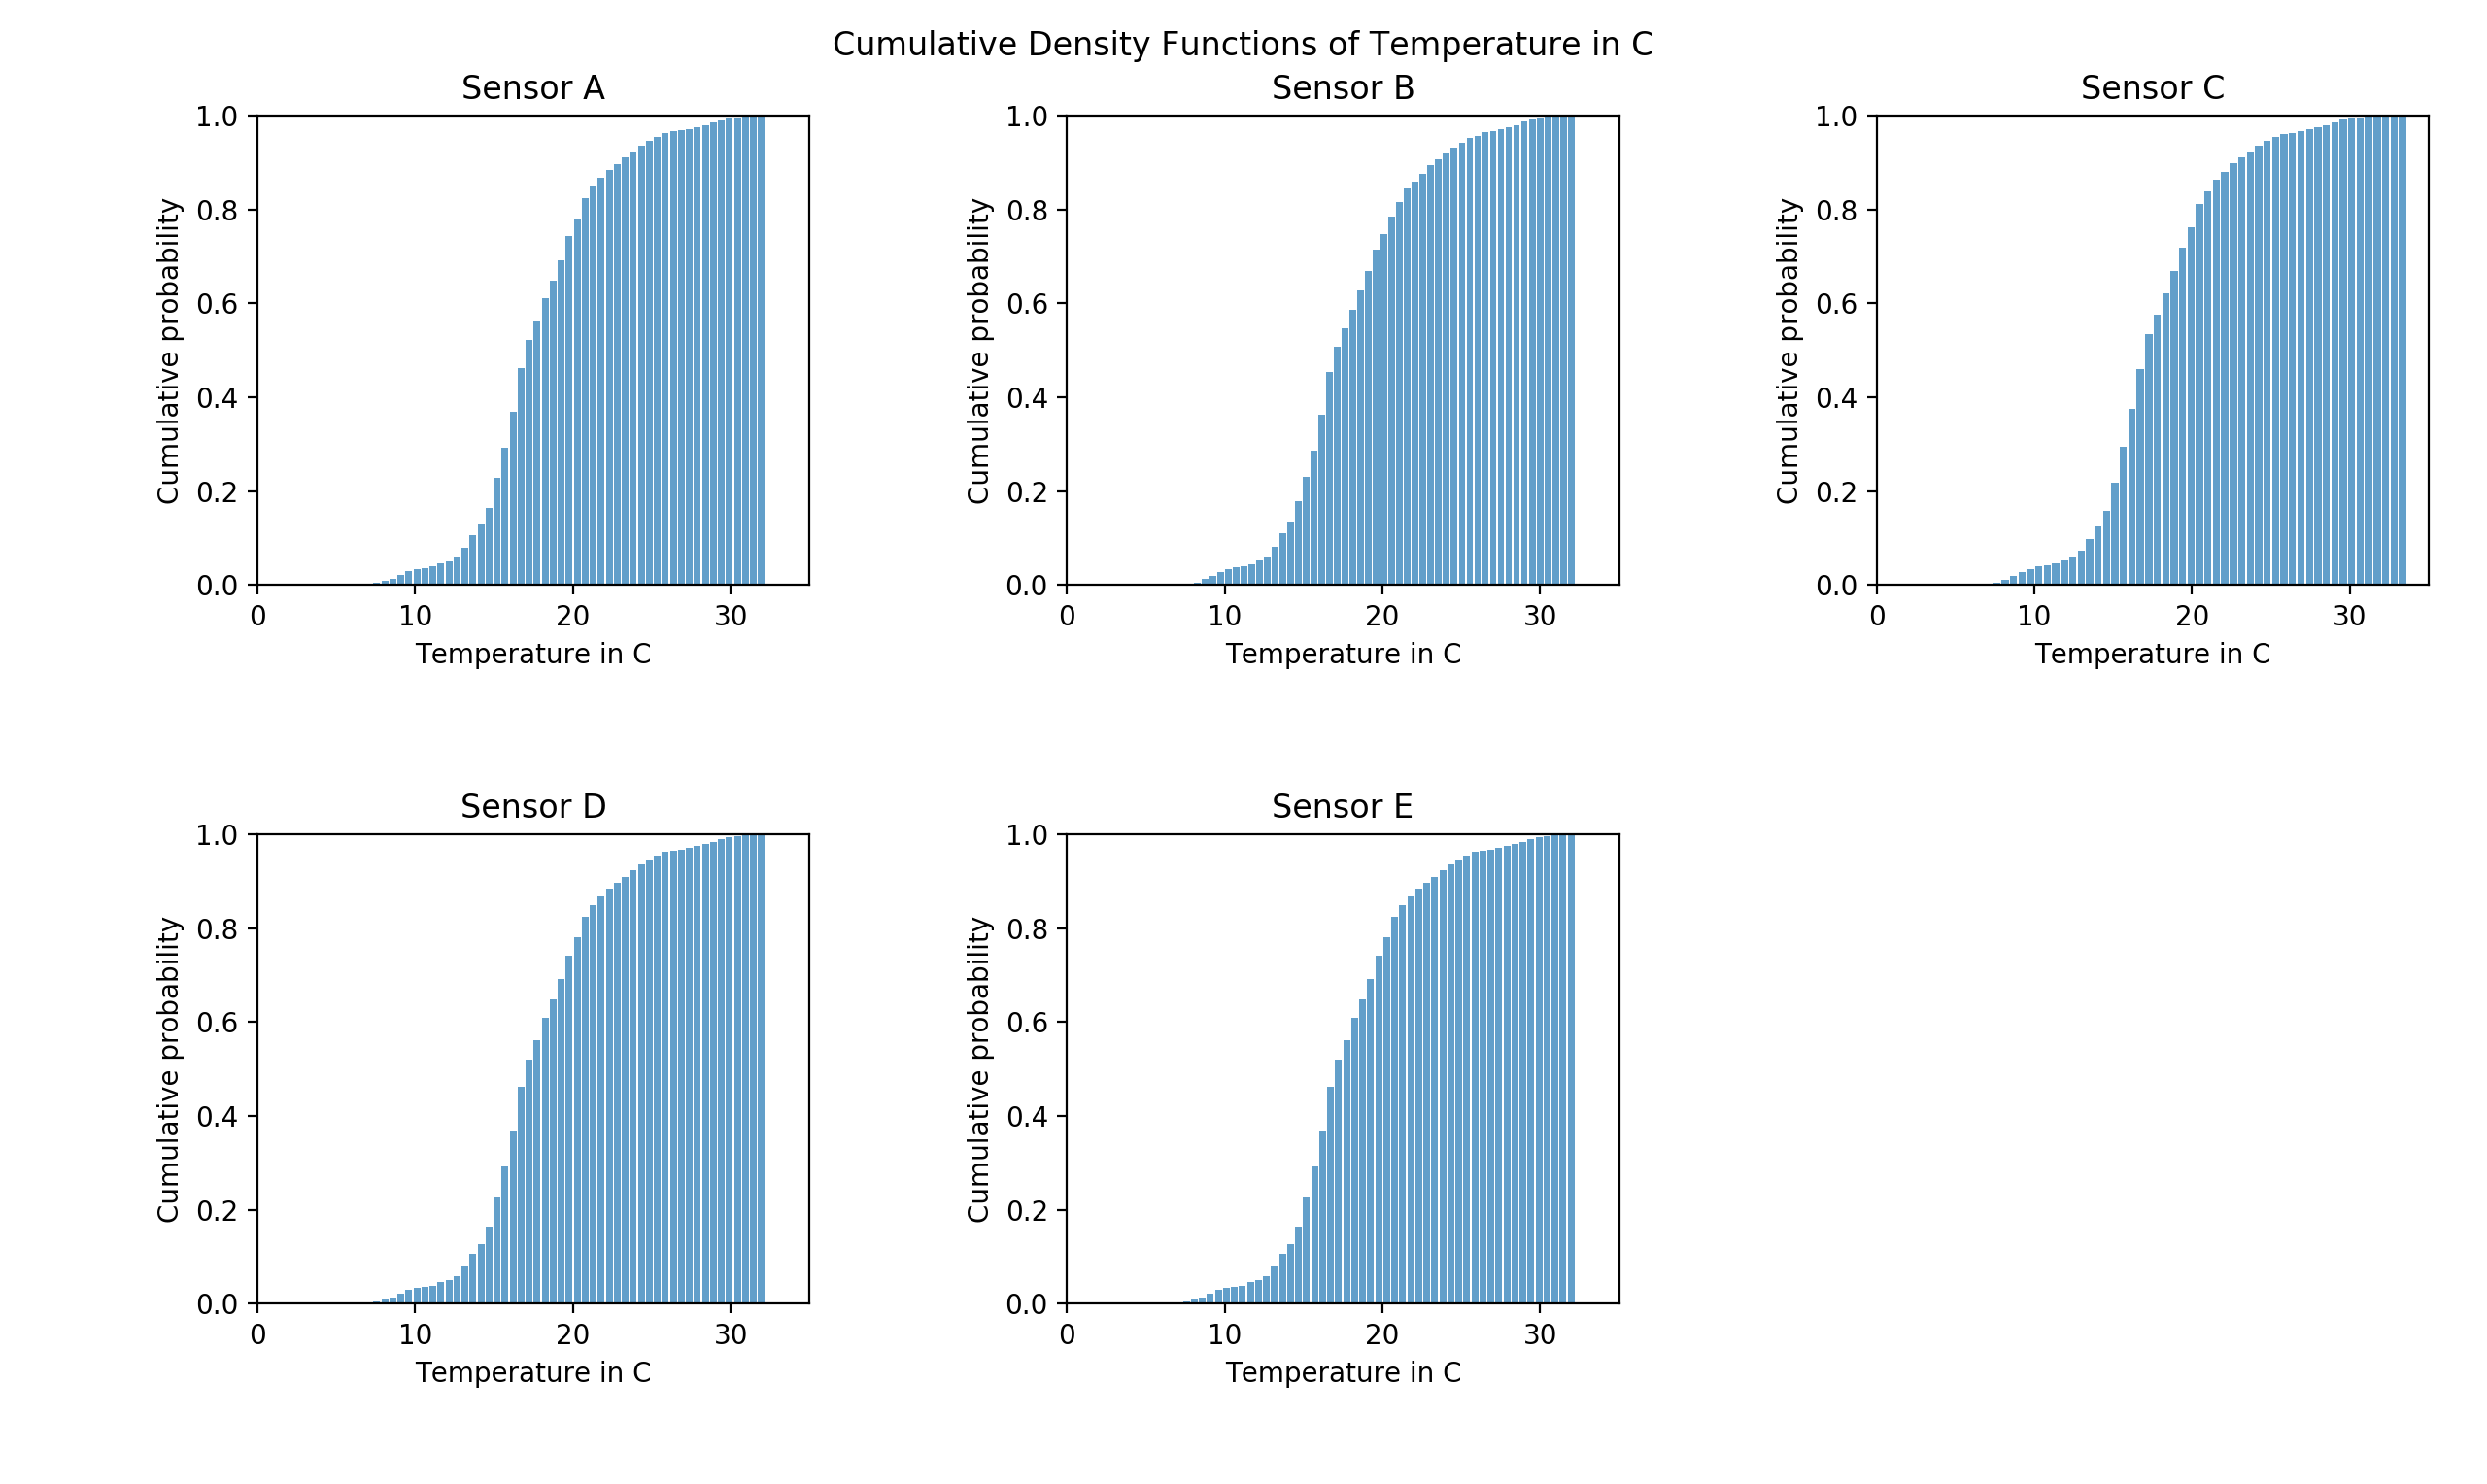
\includegraphics[width=\textwidth]{cdf_temp}
                \caption{Cumilative Density Functions of Temperature for all sensors}
            \end{figure}

            Figure 9 shows the cumulative density functions of all sensors. The functions 
            look similar for all five sensors. The cumulative probability increases the most
            in de middle (around p=0.5), which indicates a normal distribution.
            Sensor E seems to have higher temperature values, because the plot shows more 
            lines on the right side.

        \subsection{Functions Wind Speed}
            \begin{figure}[H]
                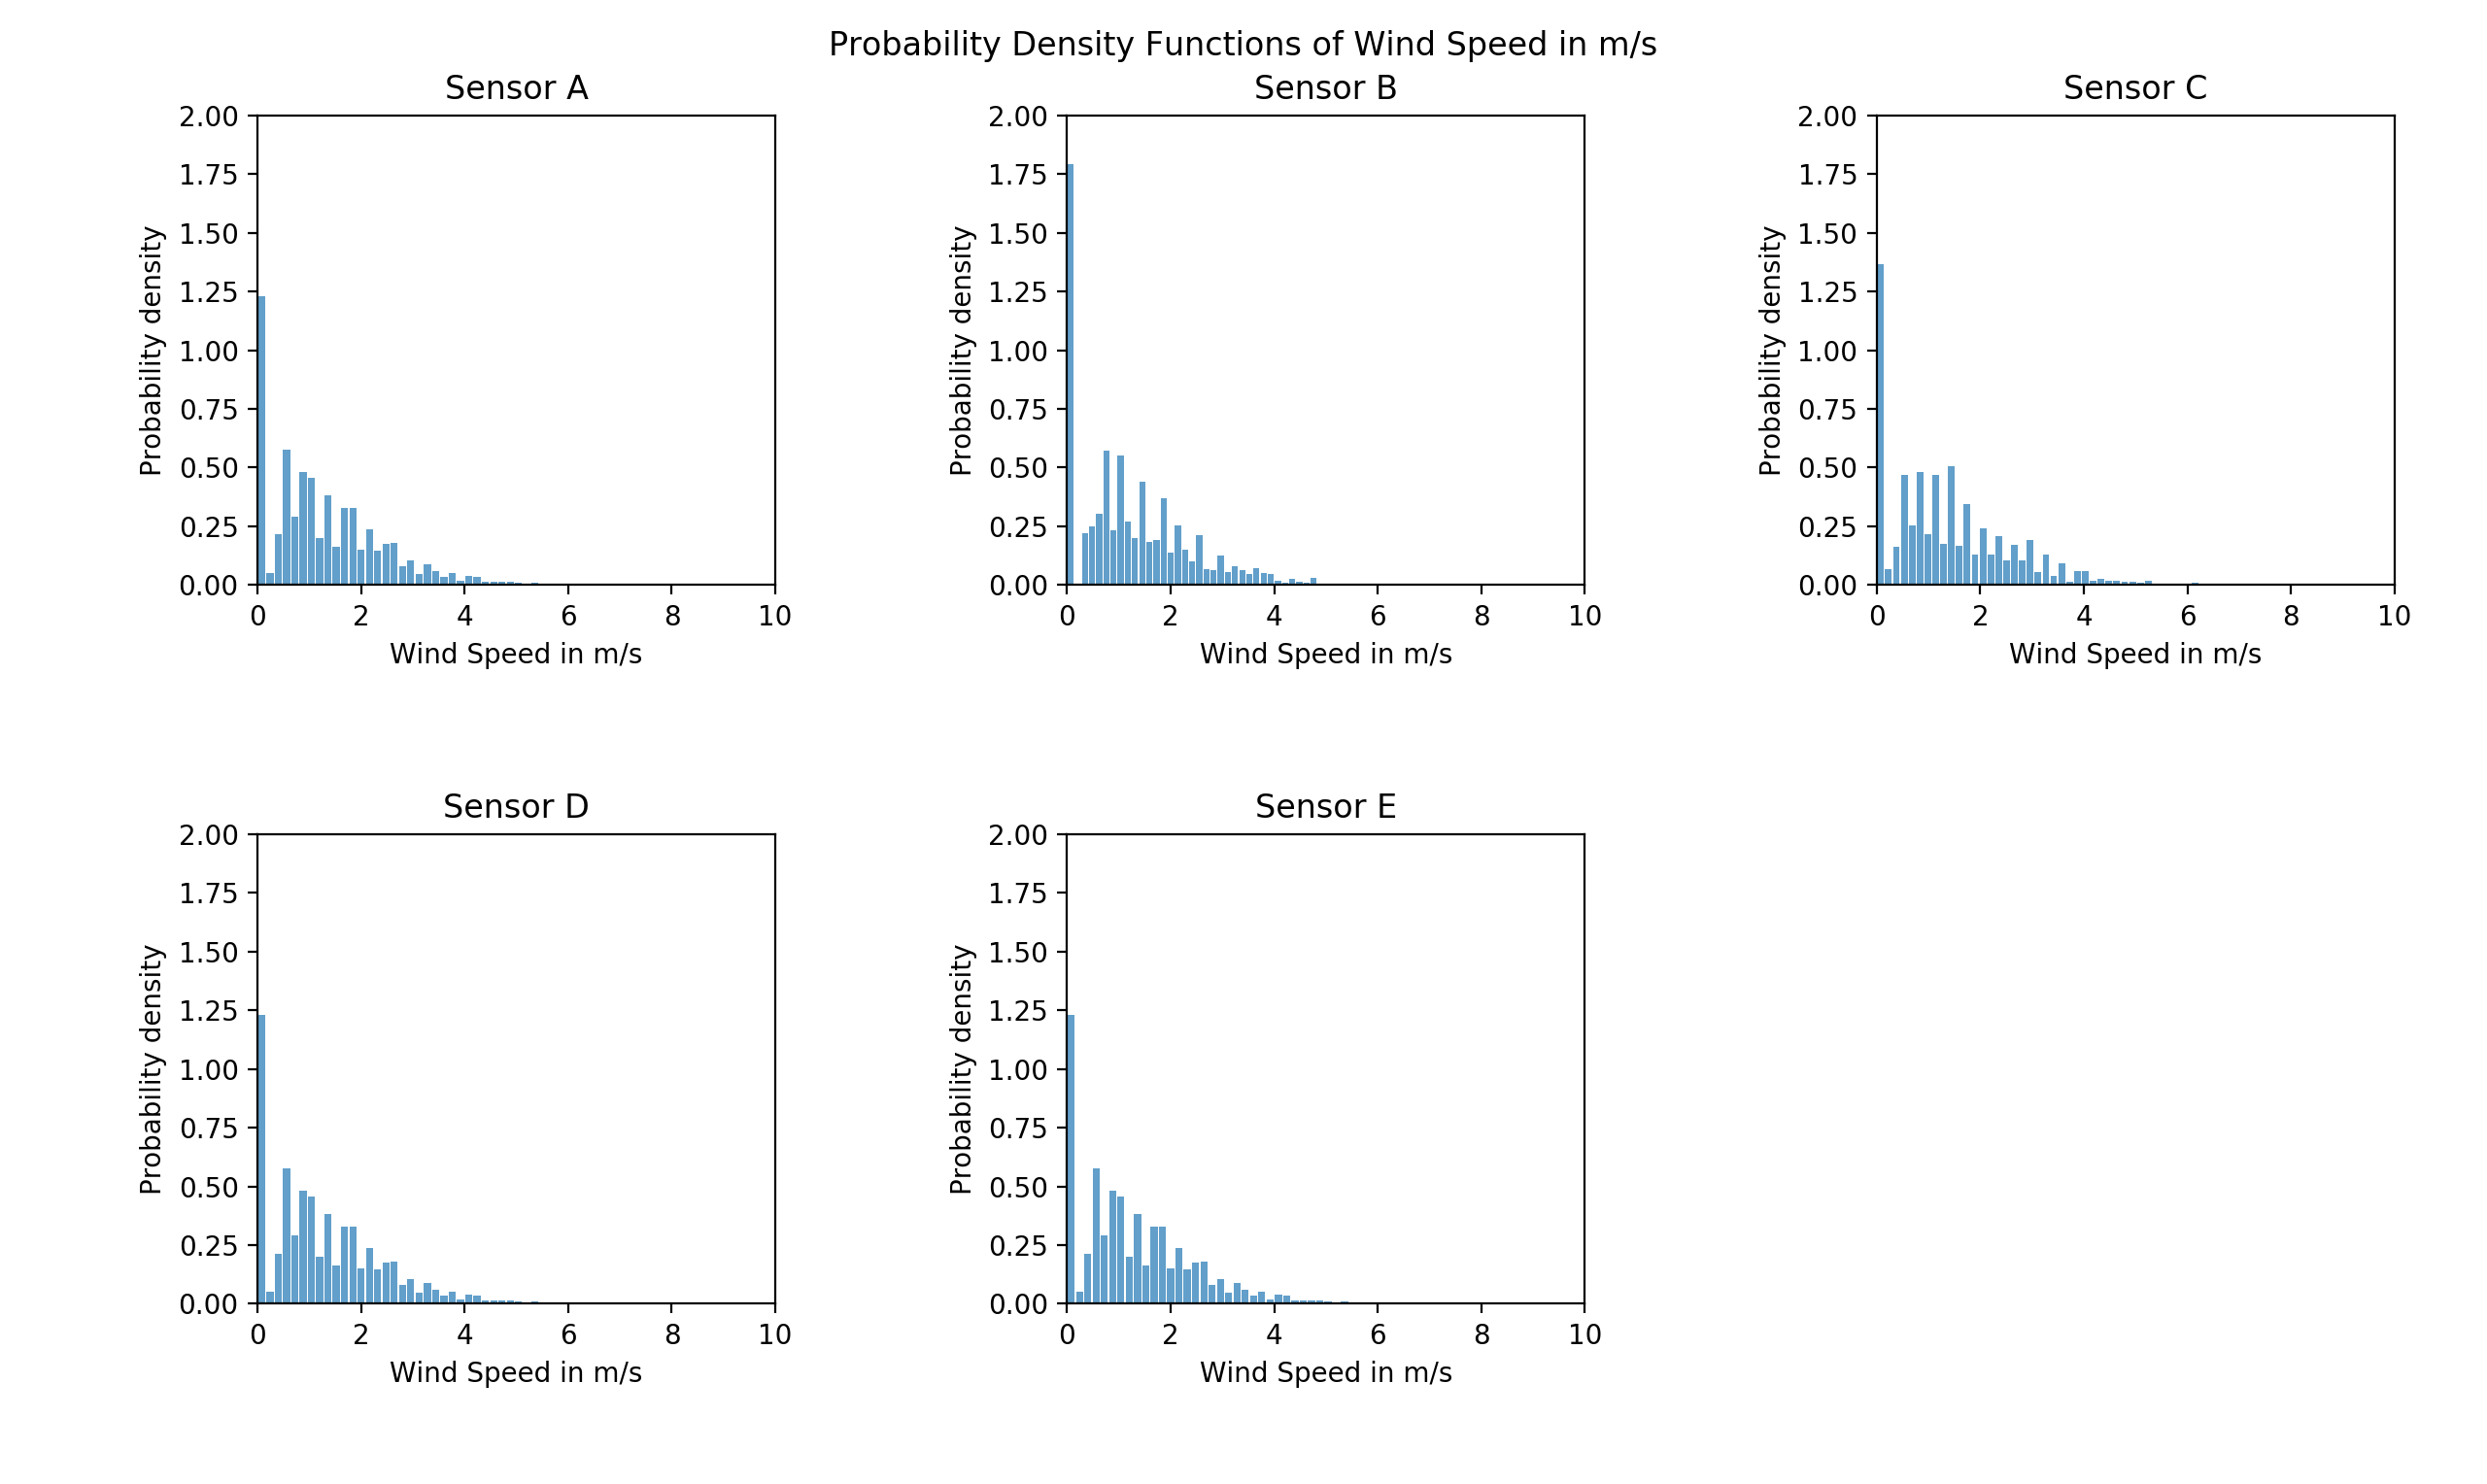
\includegraphics[width=\textwidth]{pdf_windspeed}
                \caption{Probability Density Functions of Wind Speed for all sensors}
            \end{figure}

            The PDF plots of Wind Speed (Figure 10) are very different from the Temperature
            plots. They are not normally distributed, have a very high peak at zero and 
            only a right tail. This makes sense, because having no wind occurs more 
            fequently than, for example, a wind speed of 2 m/s. Also, low wind speeds are more common
            than high wind speeds, which is why the plots are descending to the right side.
            \par There is also a big difference between the sensors. The plot of sensor E deviates 
            the most. This is mostly due to the very high frecuency of the wind speed zero. It is 
            about three times as high as the other sensors. 

            \begin{figure}[H]
                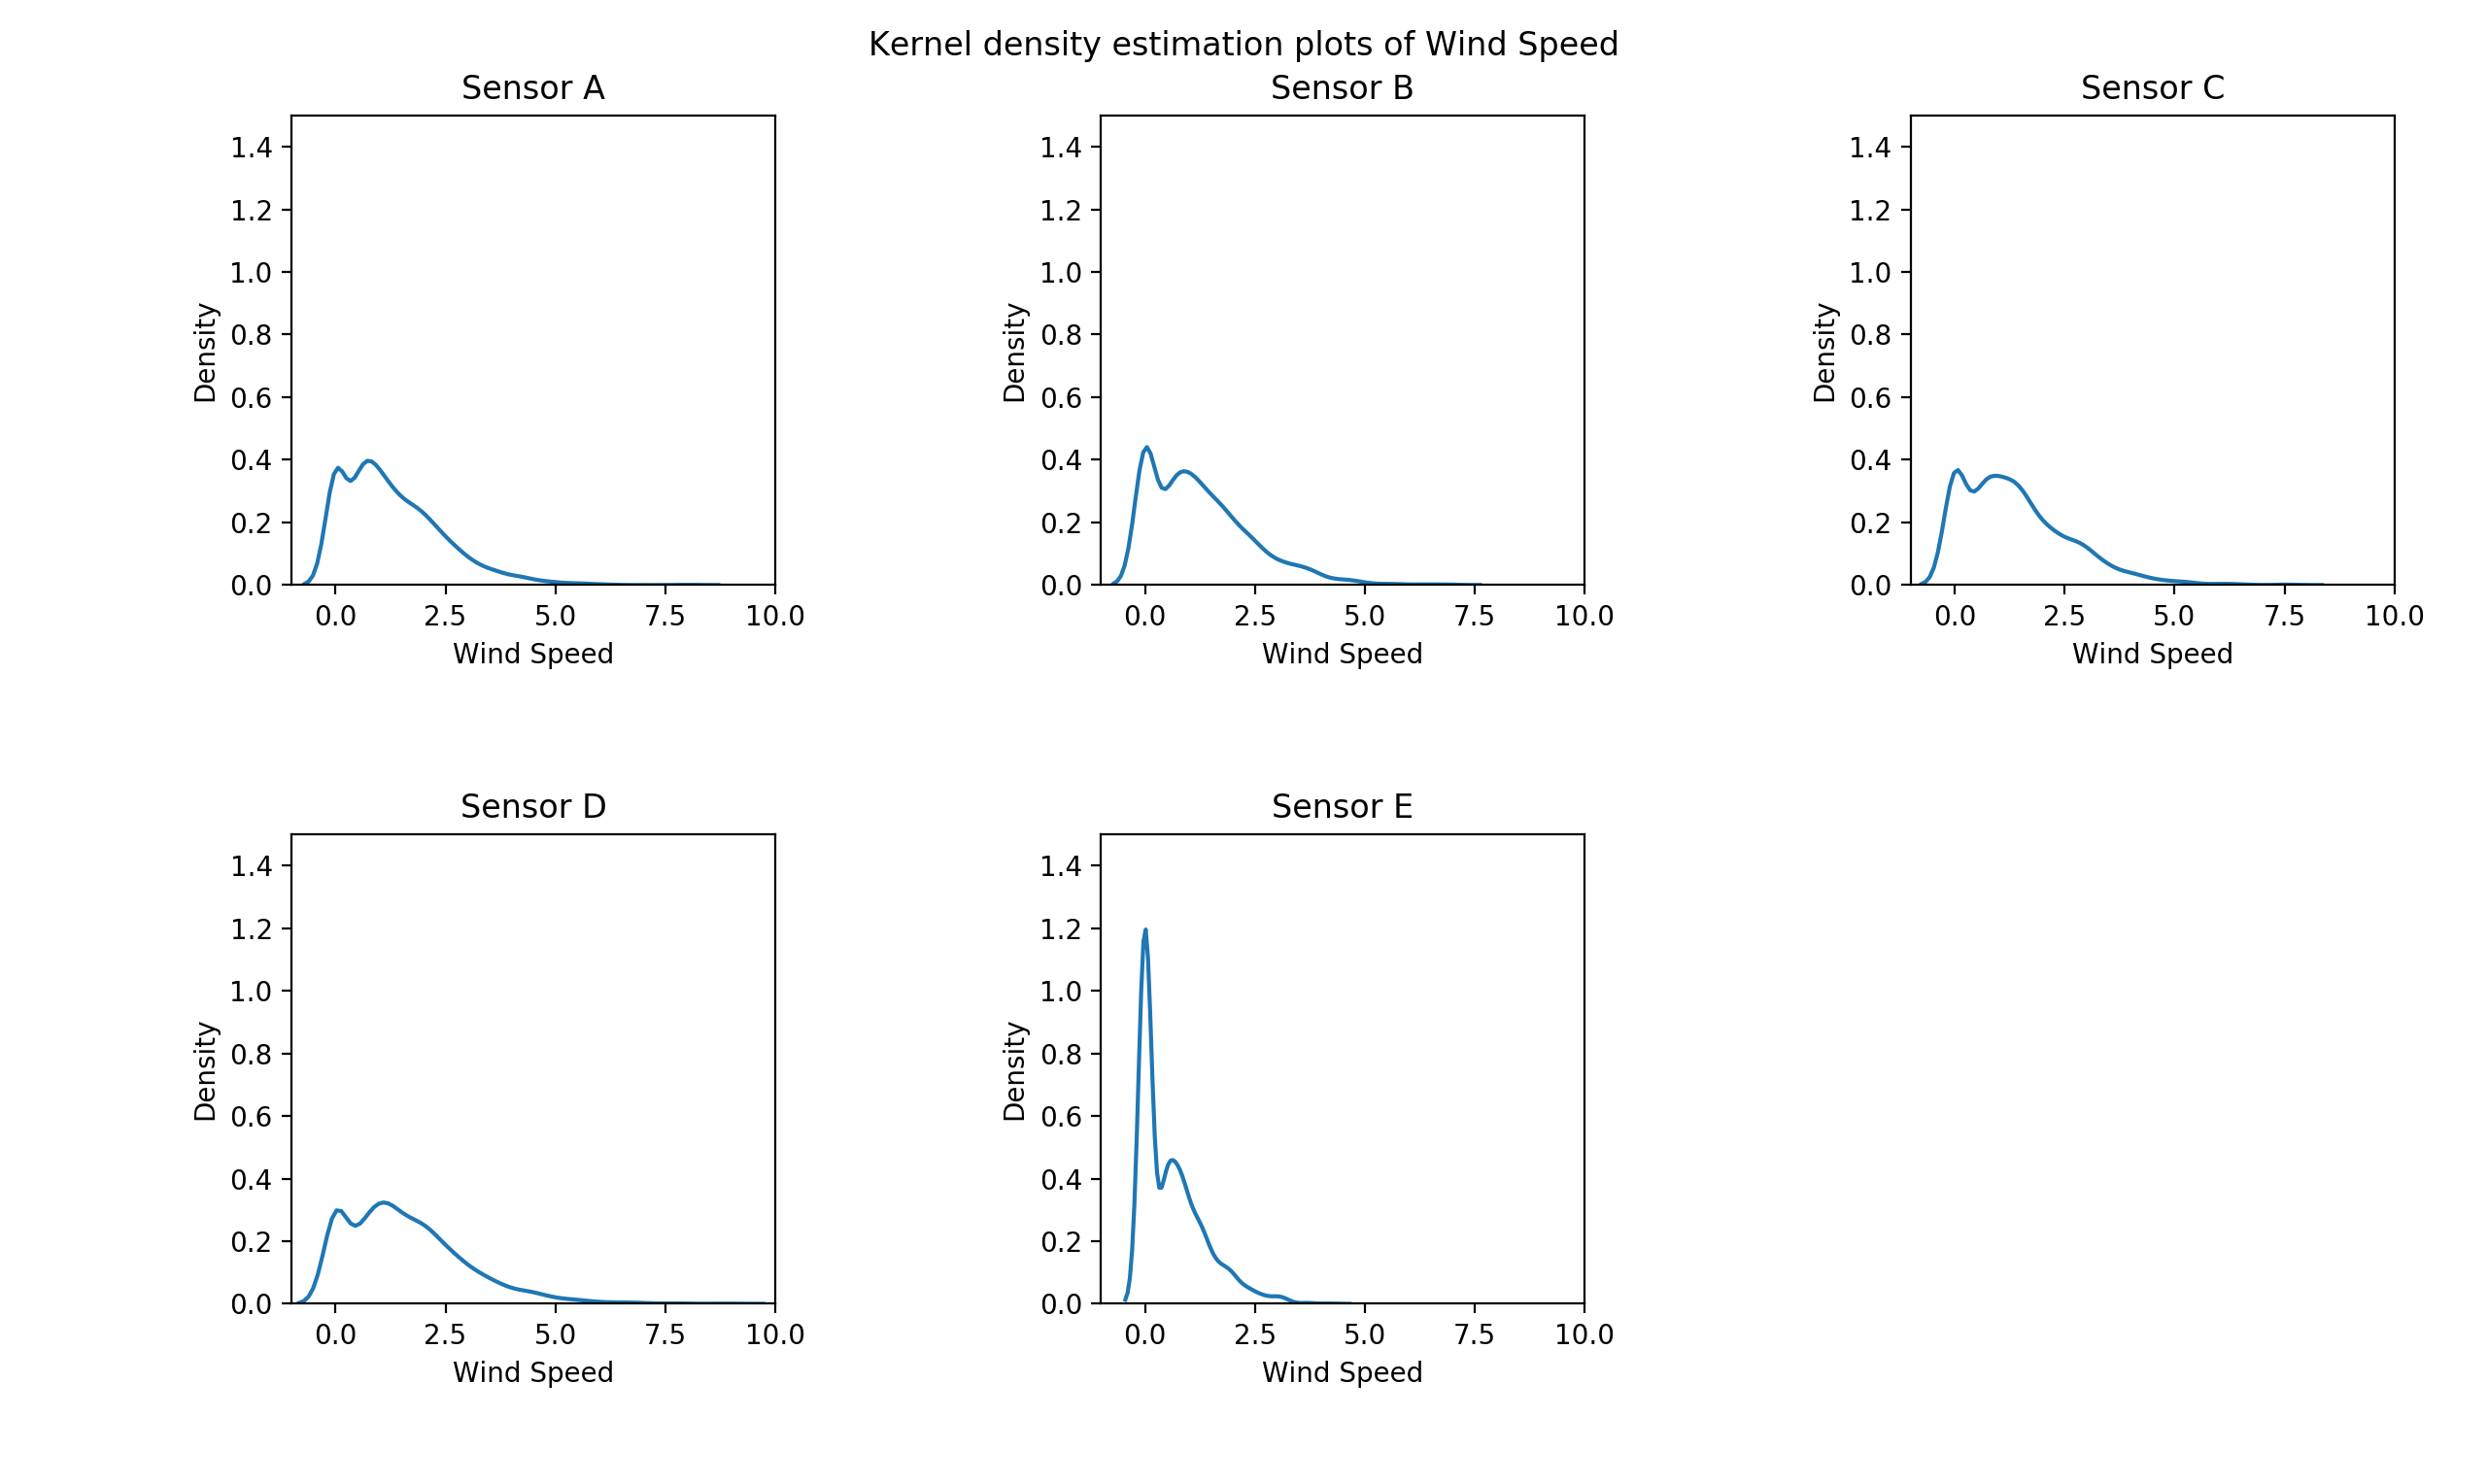
\includegraphics[width=\textwidth]{kde_windspeed}
                \caption{Kernel Density Estimation of Wind Speed for all sensors}
            \end{figure}

            In the kernel density plots (Figure 11) it can also be seen that the data is not normally distributed.
            The functions have two peaks: one for no wind and one for the wind speed with
            the highest frequency. The differences between sensors can also be seen clearly.
            The first peak of sensor E is much higher than the other sensors and the line
            stops at a lower value, because the wind speed ofsensor E has a much higher 
            frequency of zero.  
            
            



\section{A3}
    \subsection{Correlation}
        \begin{figure}[H]
            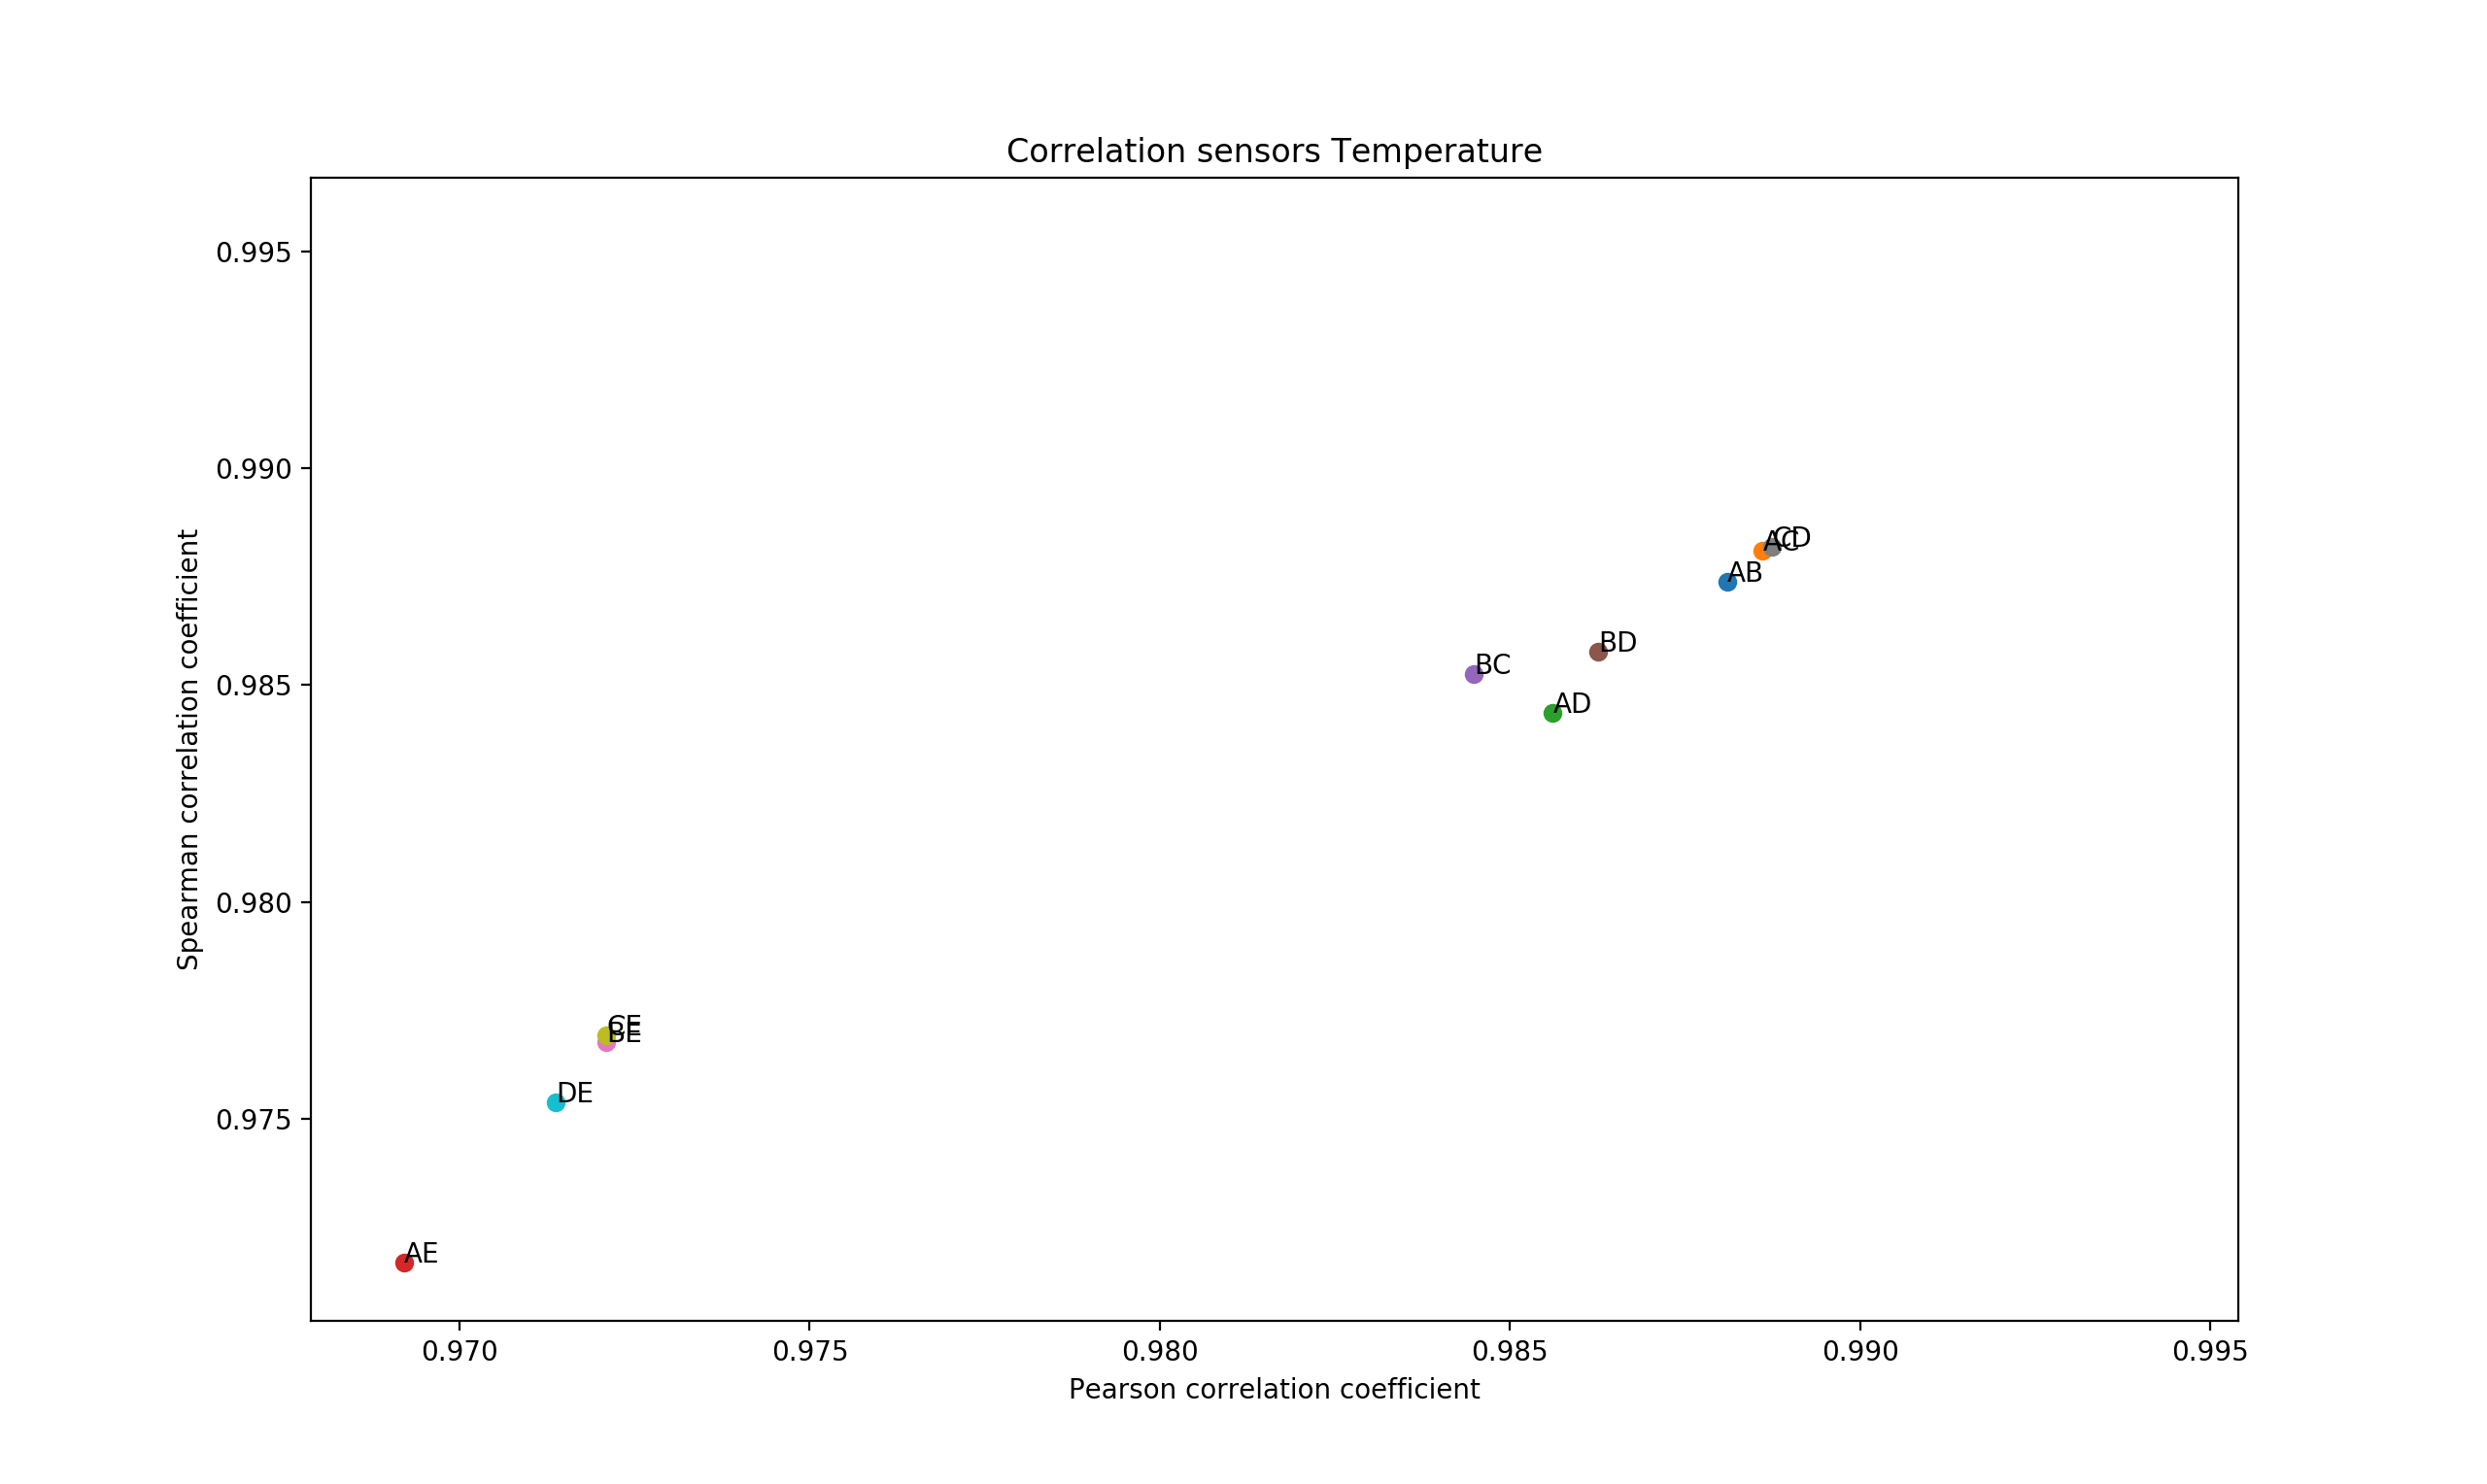
\includegraphics[width=\textwidth]{cor_temp}
            \caption{Spearman and Pearson correlation plot for all sensor combinations of Temperature}
        \end{figure}

        \begin{figure}[H]
            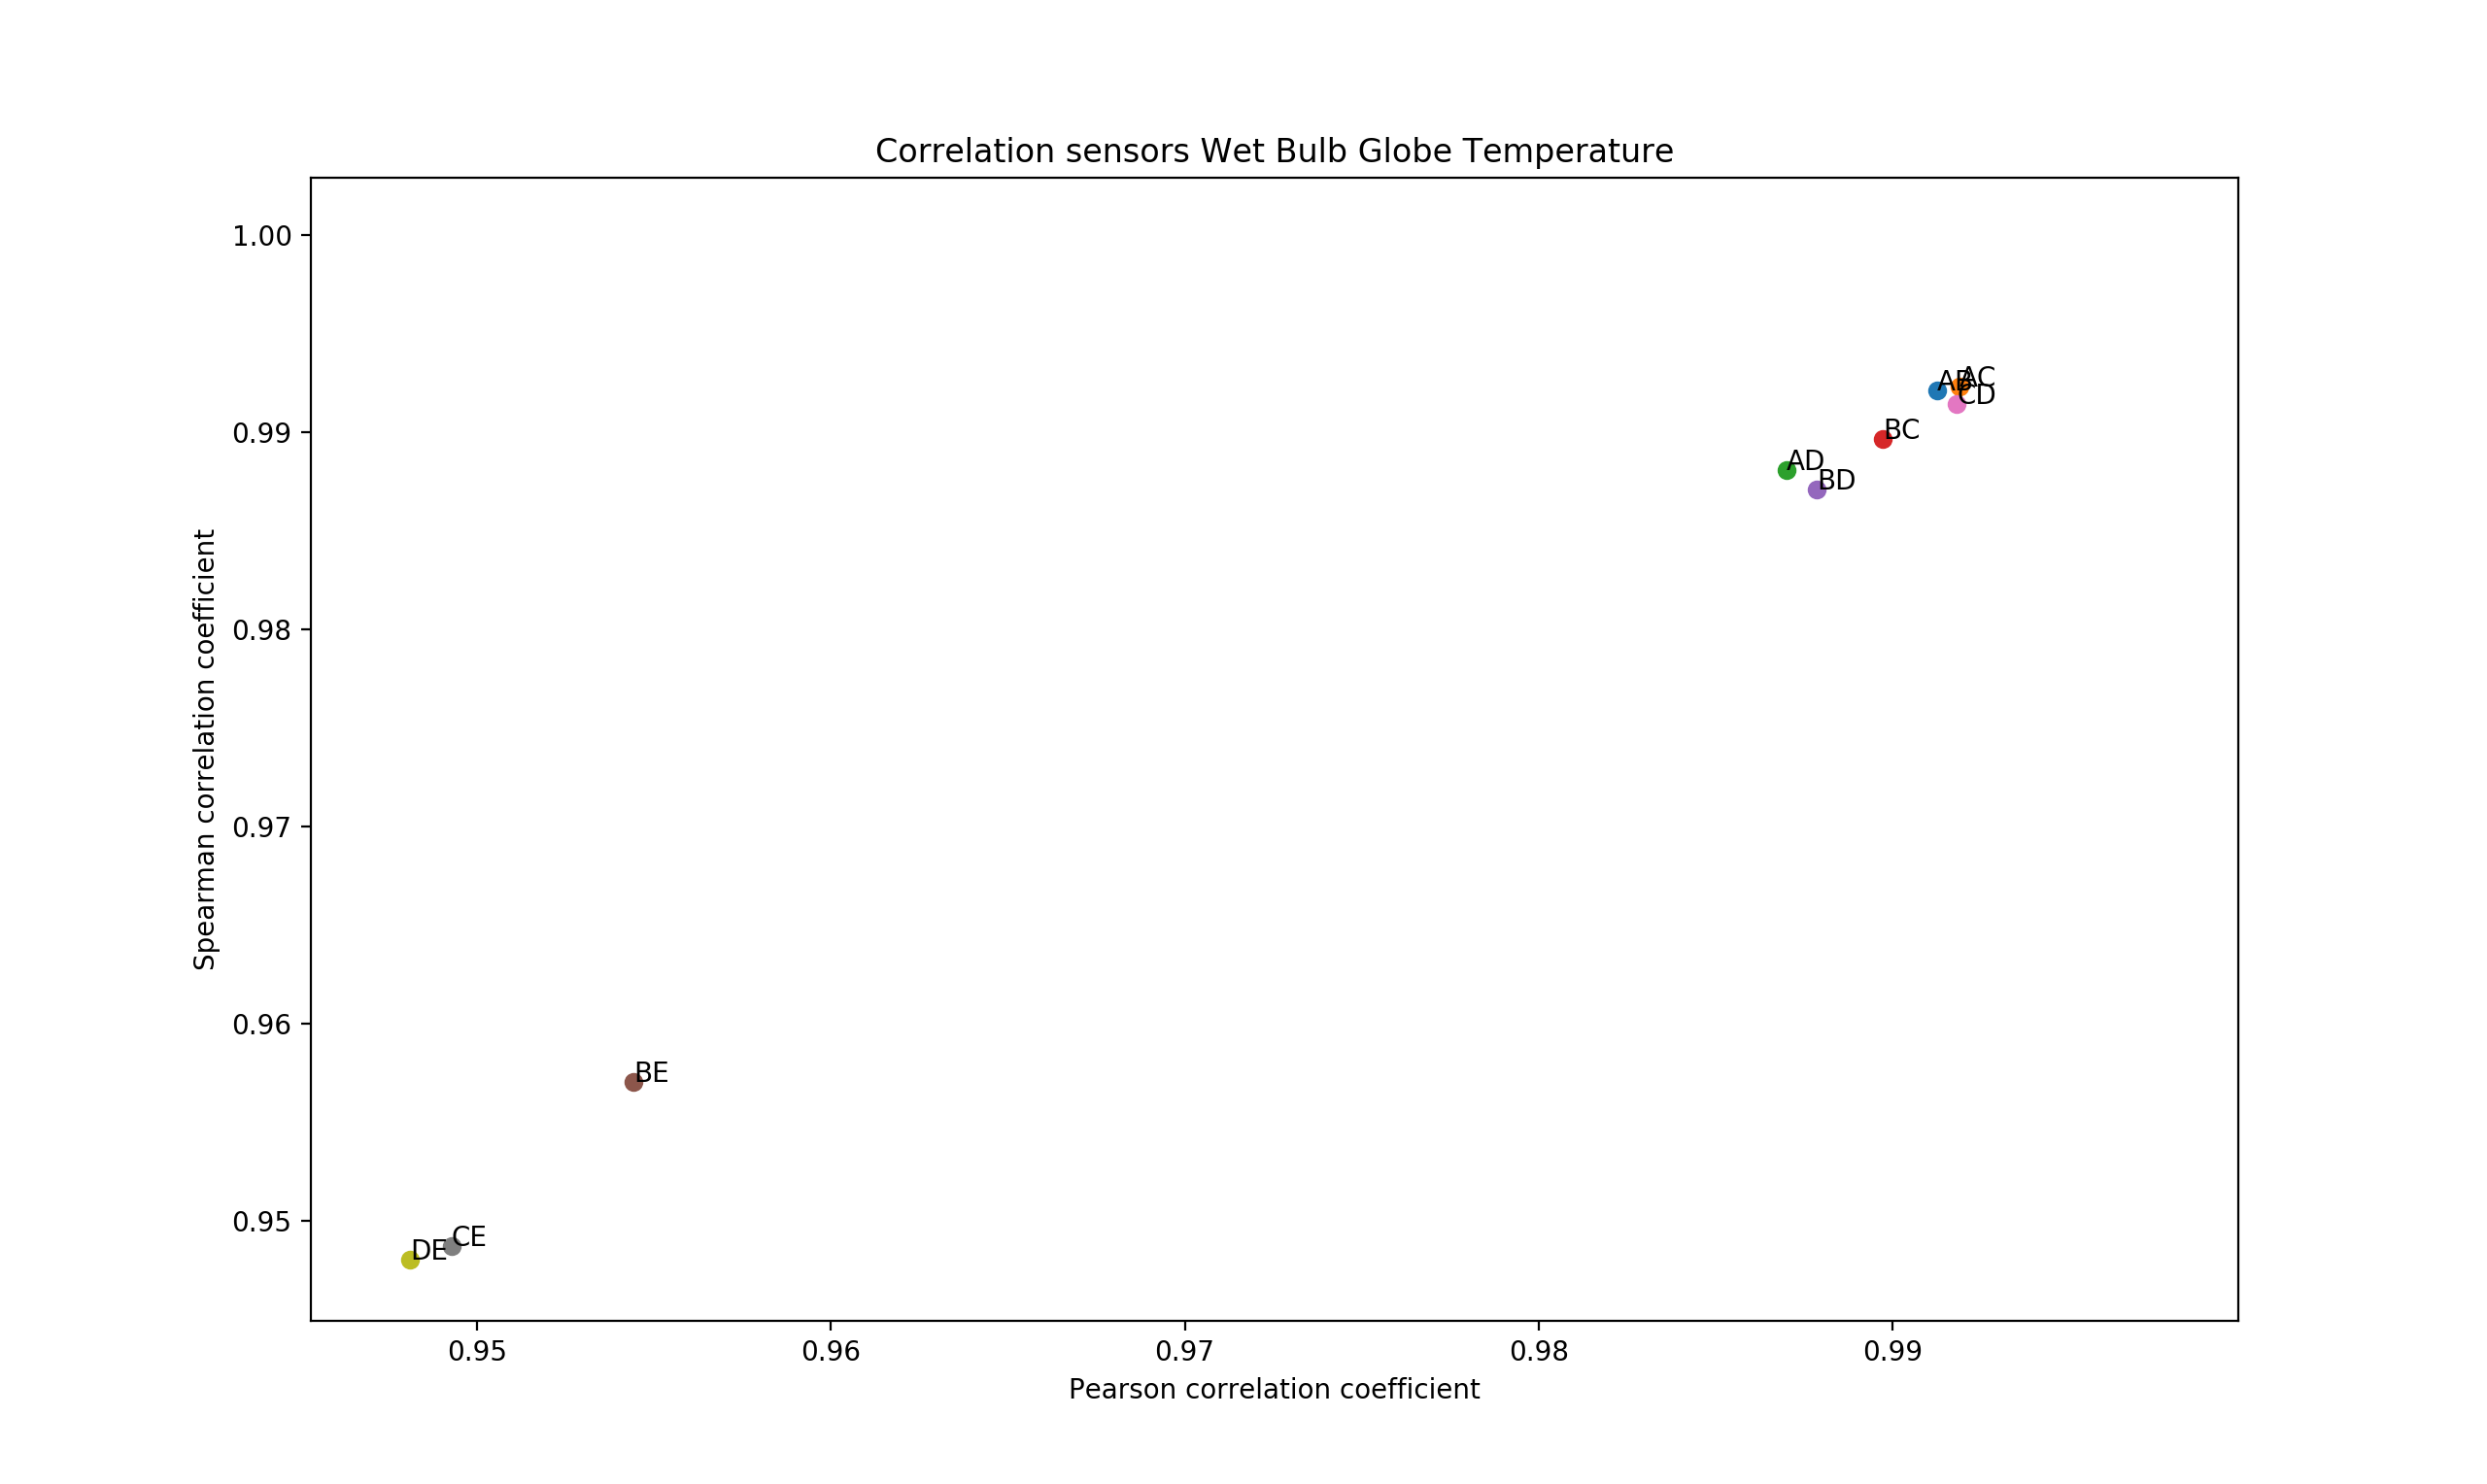
\includegraphics[width=\textwidth]{cor_wbgt}
            \caption{Spearman and Pearson correlation plot for all sensor combinations of Wet Bulb Globe Temperature}
        \end{figure}

        \begin{figure}[H]
            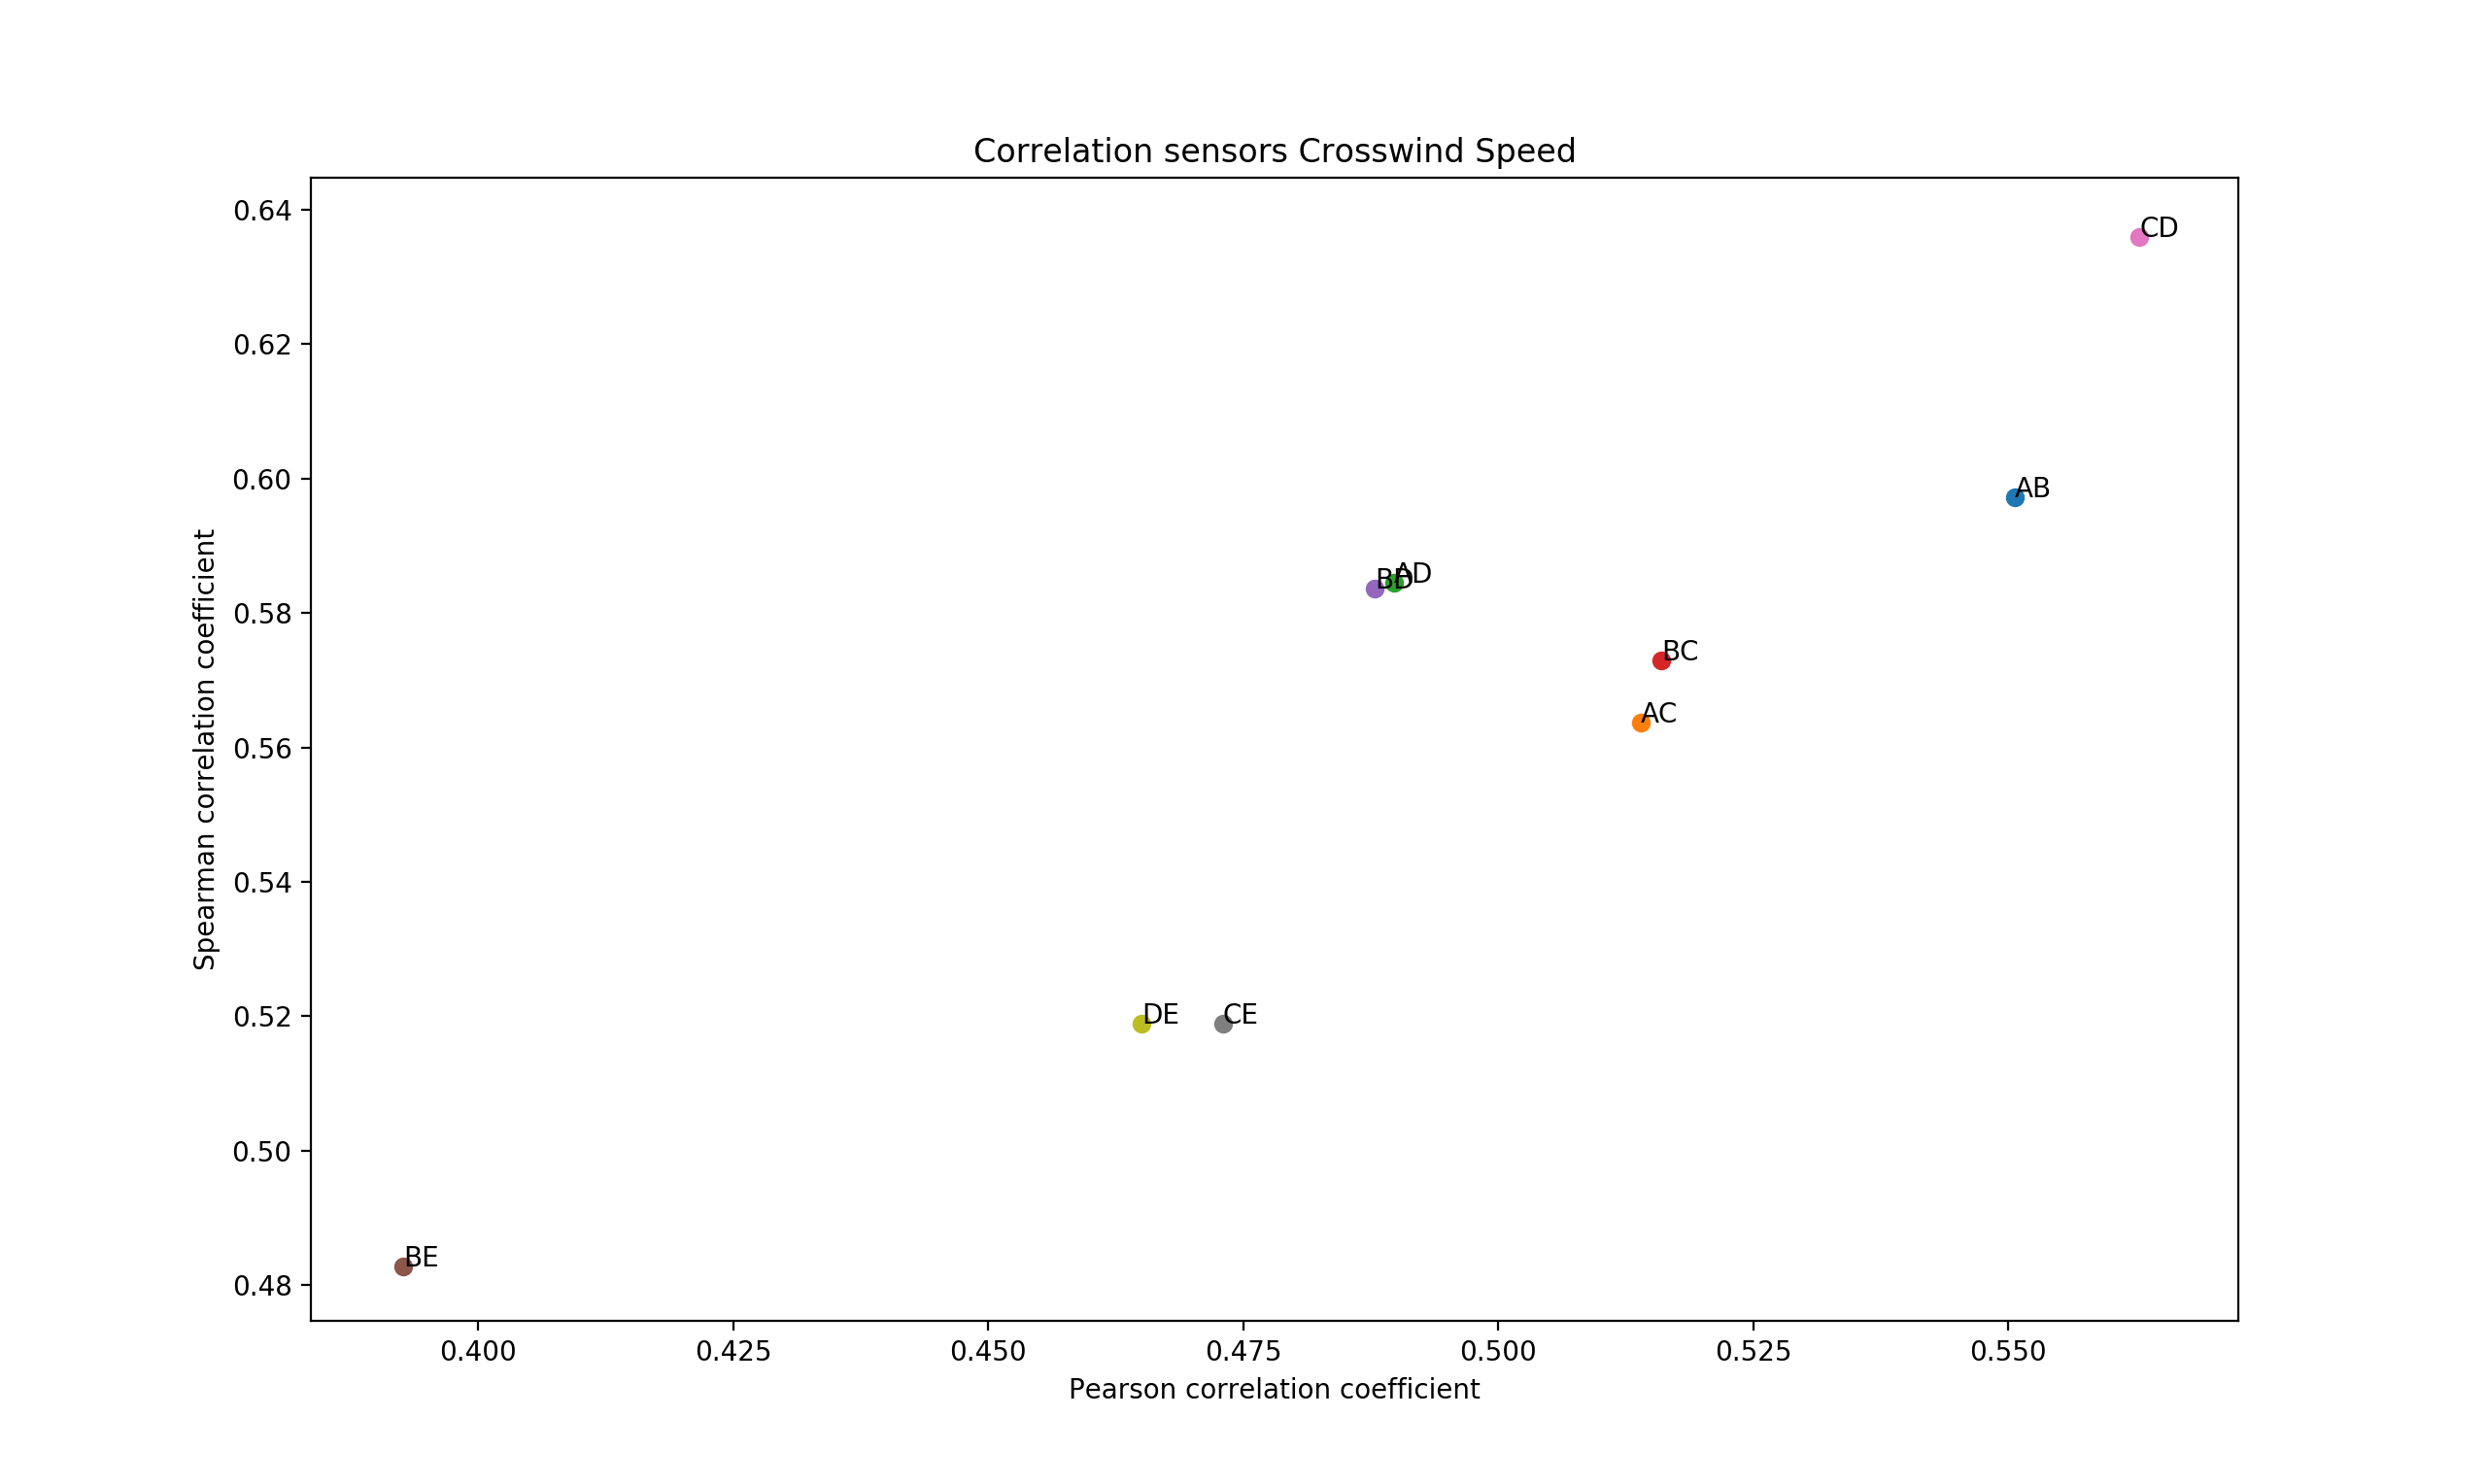
\includegraphics[width=\textwidth]{cor_cwindspeed}
            \caption{Spearman and Pearson correlation plot for all sensor combinations of Crosswind Speed}
        \end{figure}

        In the correlation plot of Temperature (Figure 12) it can be seen that all pairs are positively
        correlated. The correlation values are close to one, so there is a strong positive relationship
        between all variables. The pairs with sensor E have a relatively lower value.
        \par The correlation values of Wet Bulb Globe Temperature (Figure 13) are also high, so there is a positive
        relationship between all sensors. The pairs with sensor E are, once again, somewhat lower than
        the other pairs.
        \par The correlation values of Crosswind Speed (Figure 14) are a lot lower than correlation of 
        the other variables. However, there is still a moderate positive relationship between all 
        variable pairs. The pairs with sensor E are the three lowest correlation values and the pair
        of sensor B and sensor E is clearly the lowest.
    
    \subsection{Sensor locations} 
        \begin{figure}[H]
            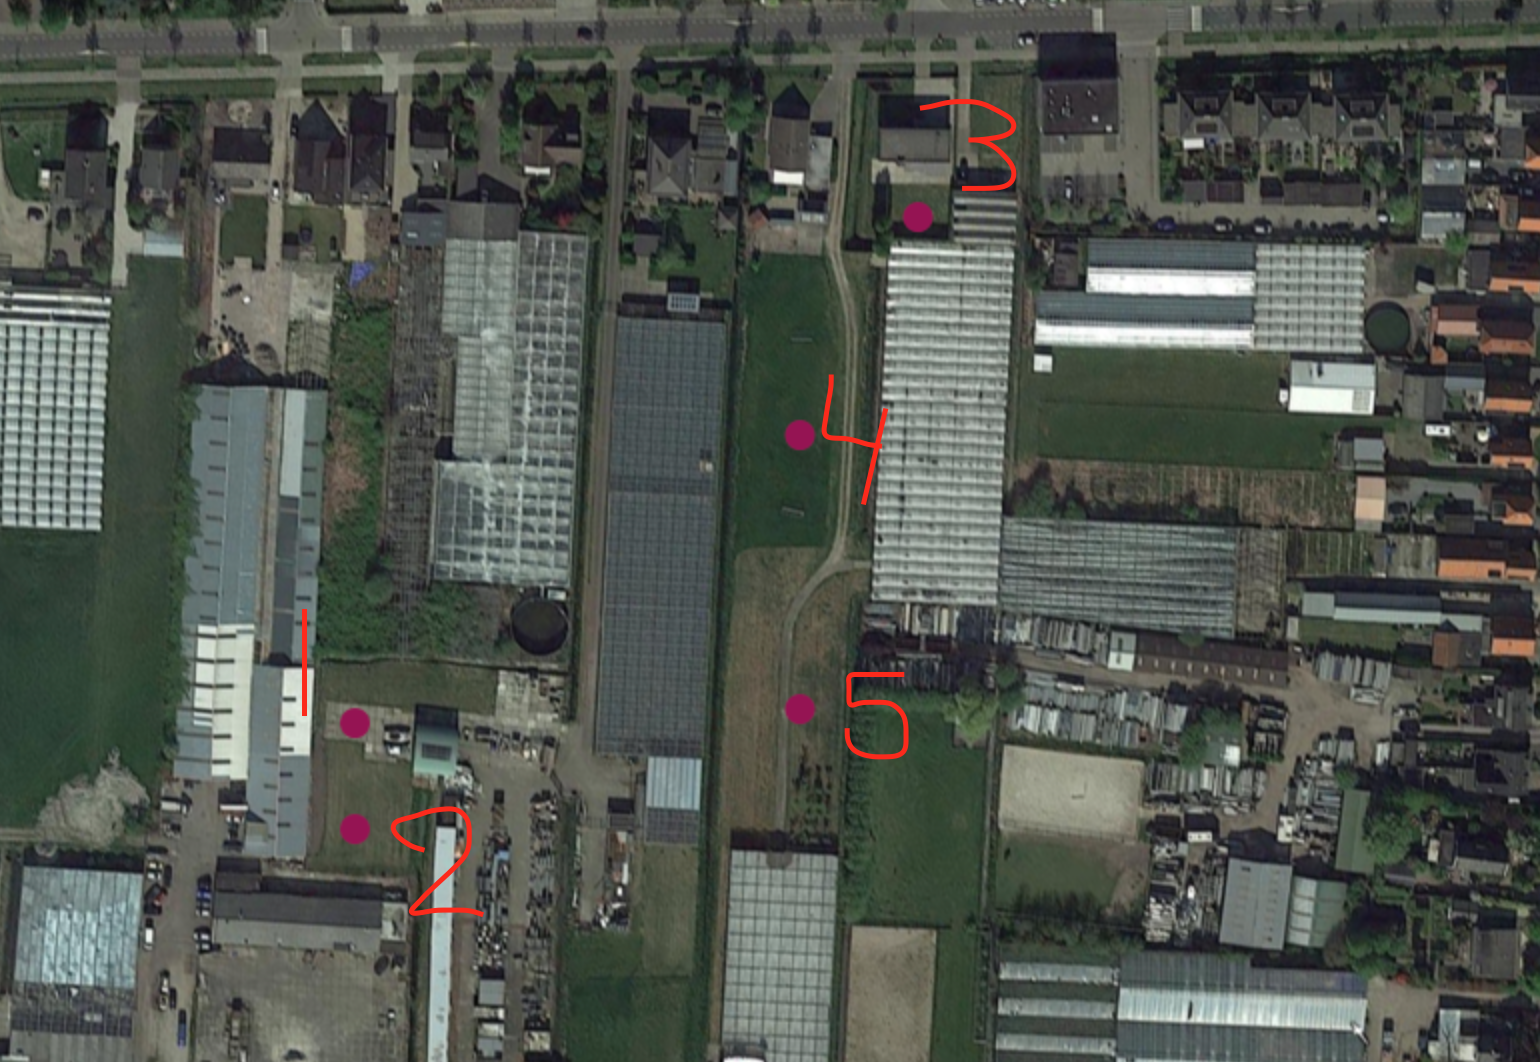
\includegraphics[width=\textwidth]{sensor_locations.png}
            \caption{Sensor locations by number}
        \end{figure}

        In Figure 15 the five potential locations of the sensors are shown. As was clear in the
        last section, sensor E differs the most from the other sensors. Therefore, its location 
        would lay the furthest away, which is location 3. Furthermore, the pair of 
        sensors C and D had the highest correlations for all variables, so they should lay the closest 
        together, which are locations 1 and 2. This leaves locations 4 and 5 for sensors A and B. This
        seems correct, because the correlation between A and B are the second highest and locations 4 and 
        5 are the second closest together. The AE pair has a lower correlation for variables Temperature 
        and WBGT compared to pair BE. Only for Crosswind Speed the correlation of AE is higher than 
        BE, but because wind is so variable, the temperature variables are valued more. So Sensor B
        is hypothesized to be situated at location 4 and sensor A at location 5, because B has a higher 
        correlation with E. Because location 1
        is the closest to sensor A, the sensor that is situated there should be more correlated to A
        than the sensor at location 2. Although is is very close, sensor C is more strongly correlated
        with sensor A than sensor D for variables Temperature and WBGT. For variable Crosswind Speed,
        pair AD is slightly more correlated, but as mentioned before, this variable is less valued 
        due to its high variability. So, sensor C is estimated to be situated at location 1 and 
        sensor D is situated at location 2. The hypothesized locations are shown in Figure 16.


        \begin{figure}[H]
            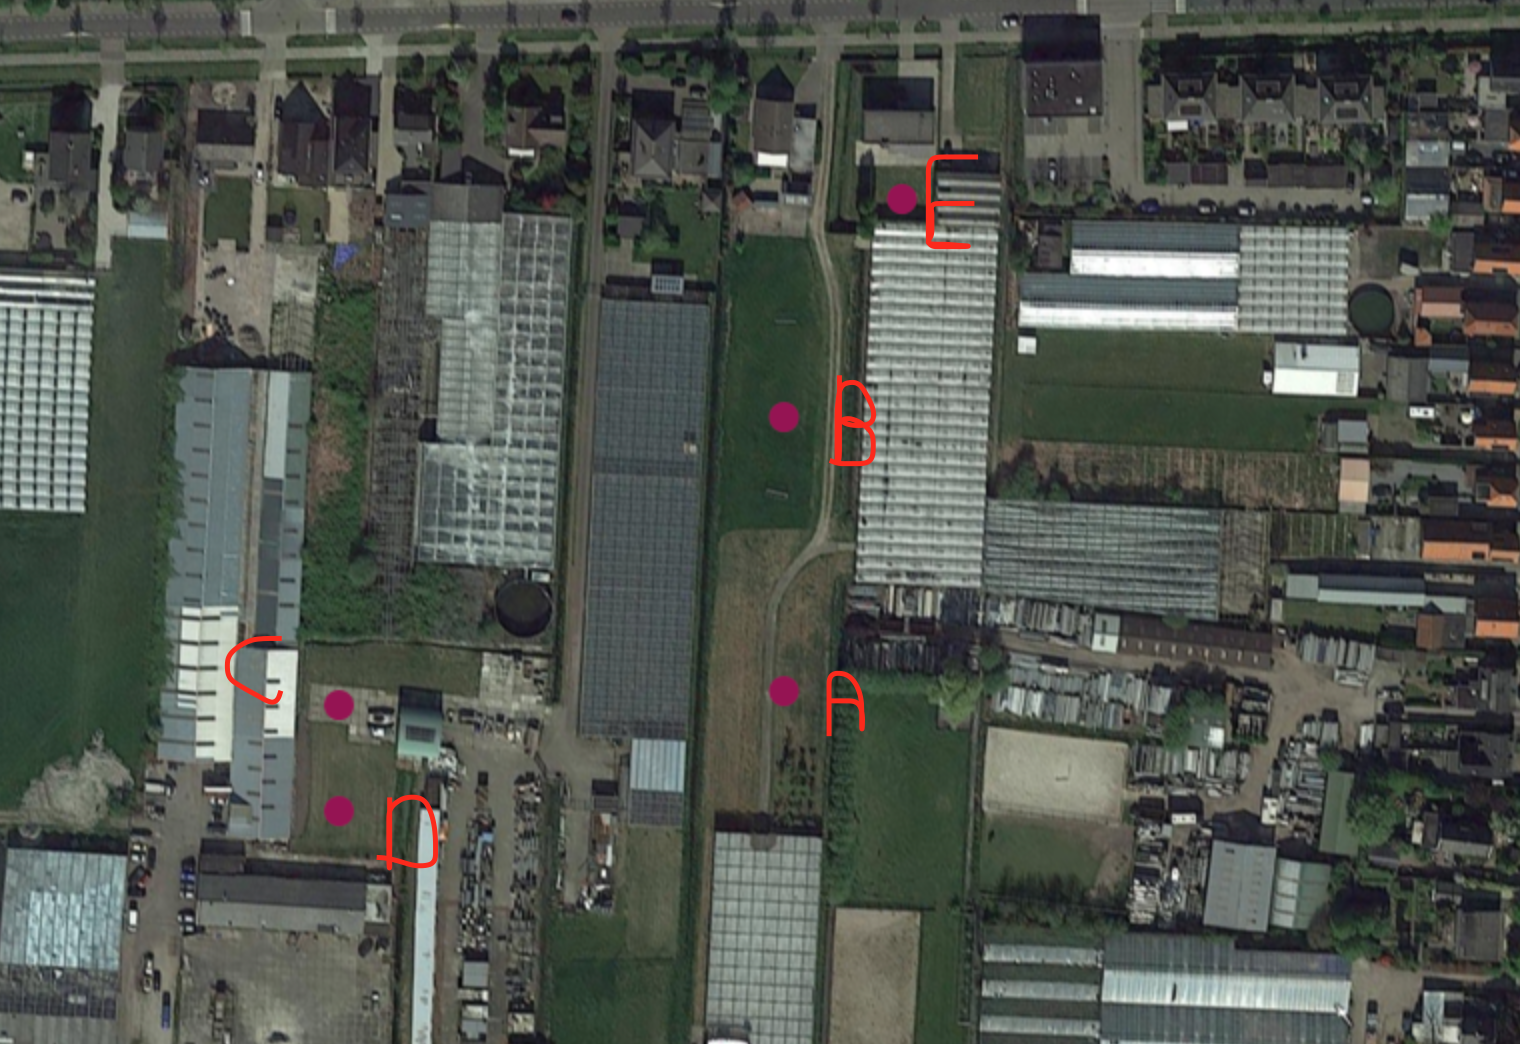
\includegraphics[width=\textwidth]{hypo_locations.png}
            \caption{Hypothesized locations of sensors}
        \end{figure}

\section{A4}
    \subsection{Cumulative Density Functions}
        \begin{figure}[H]
            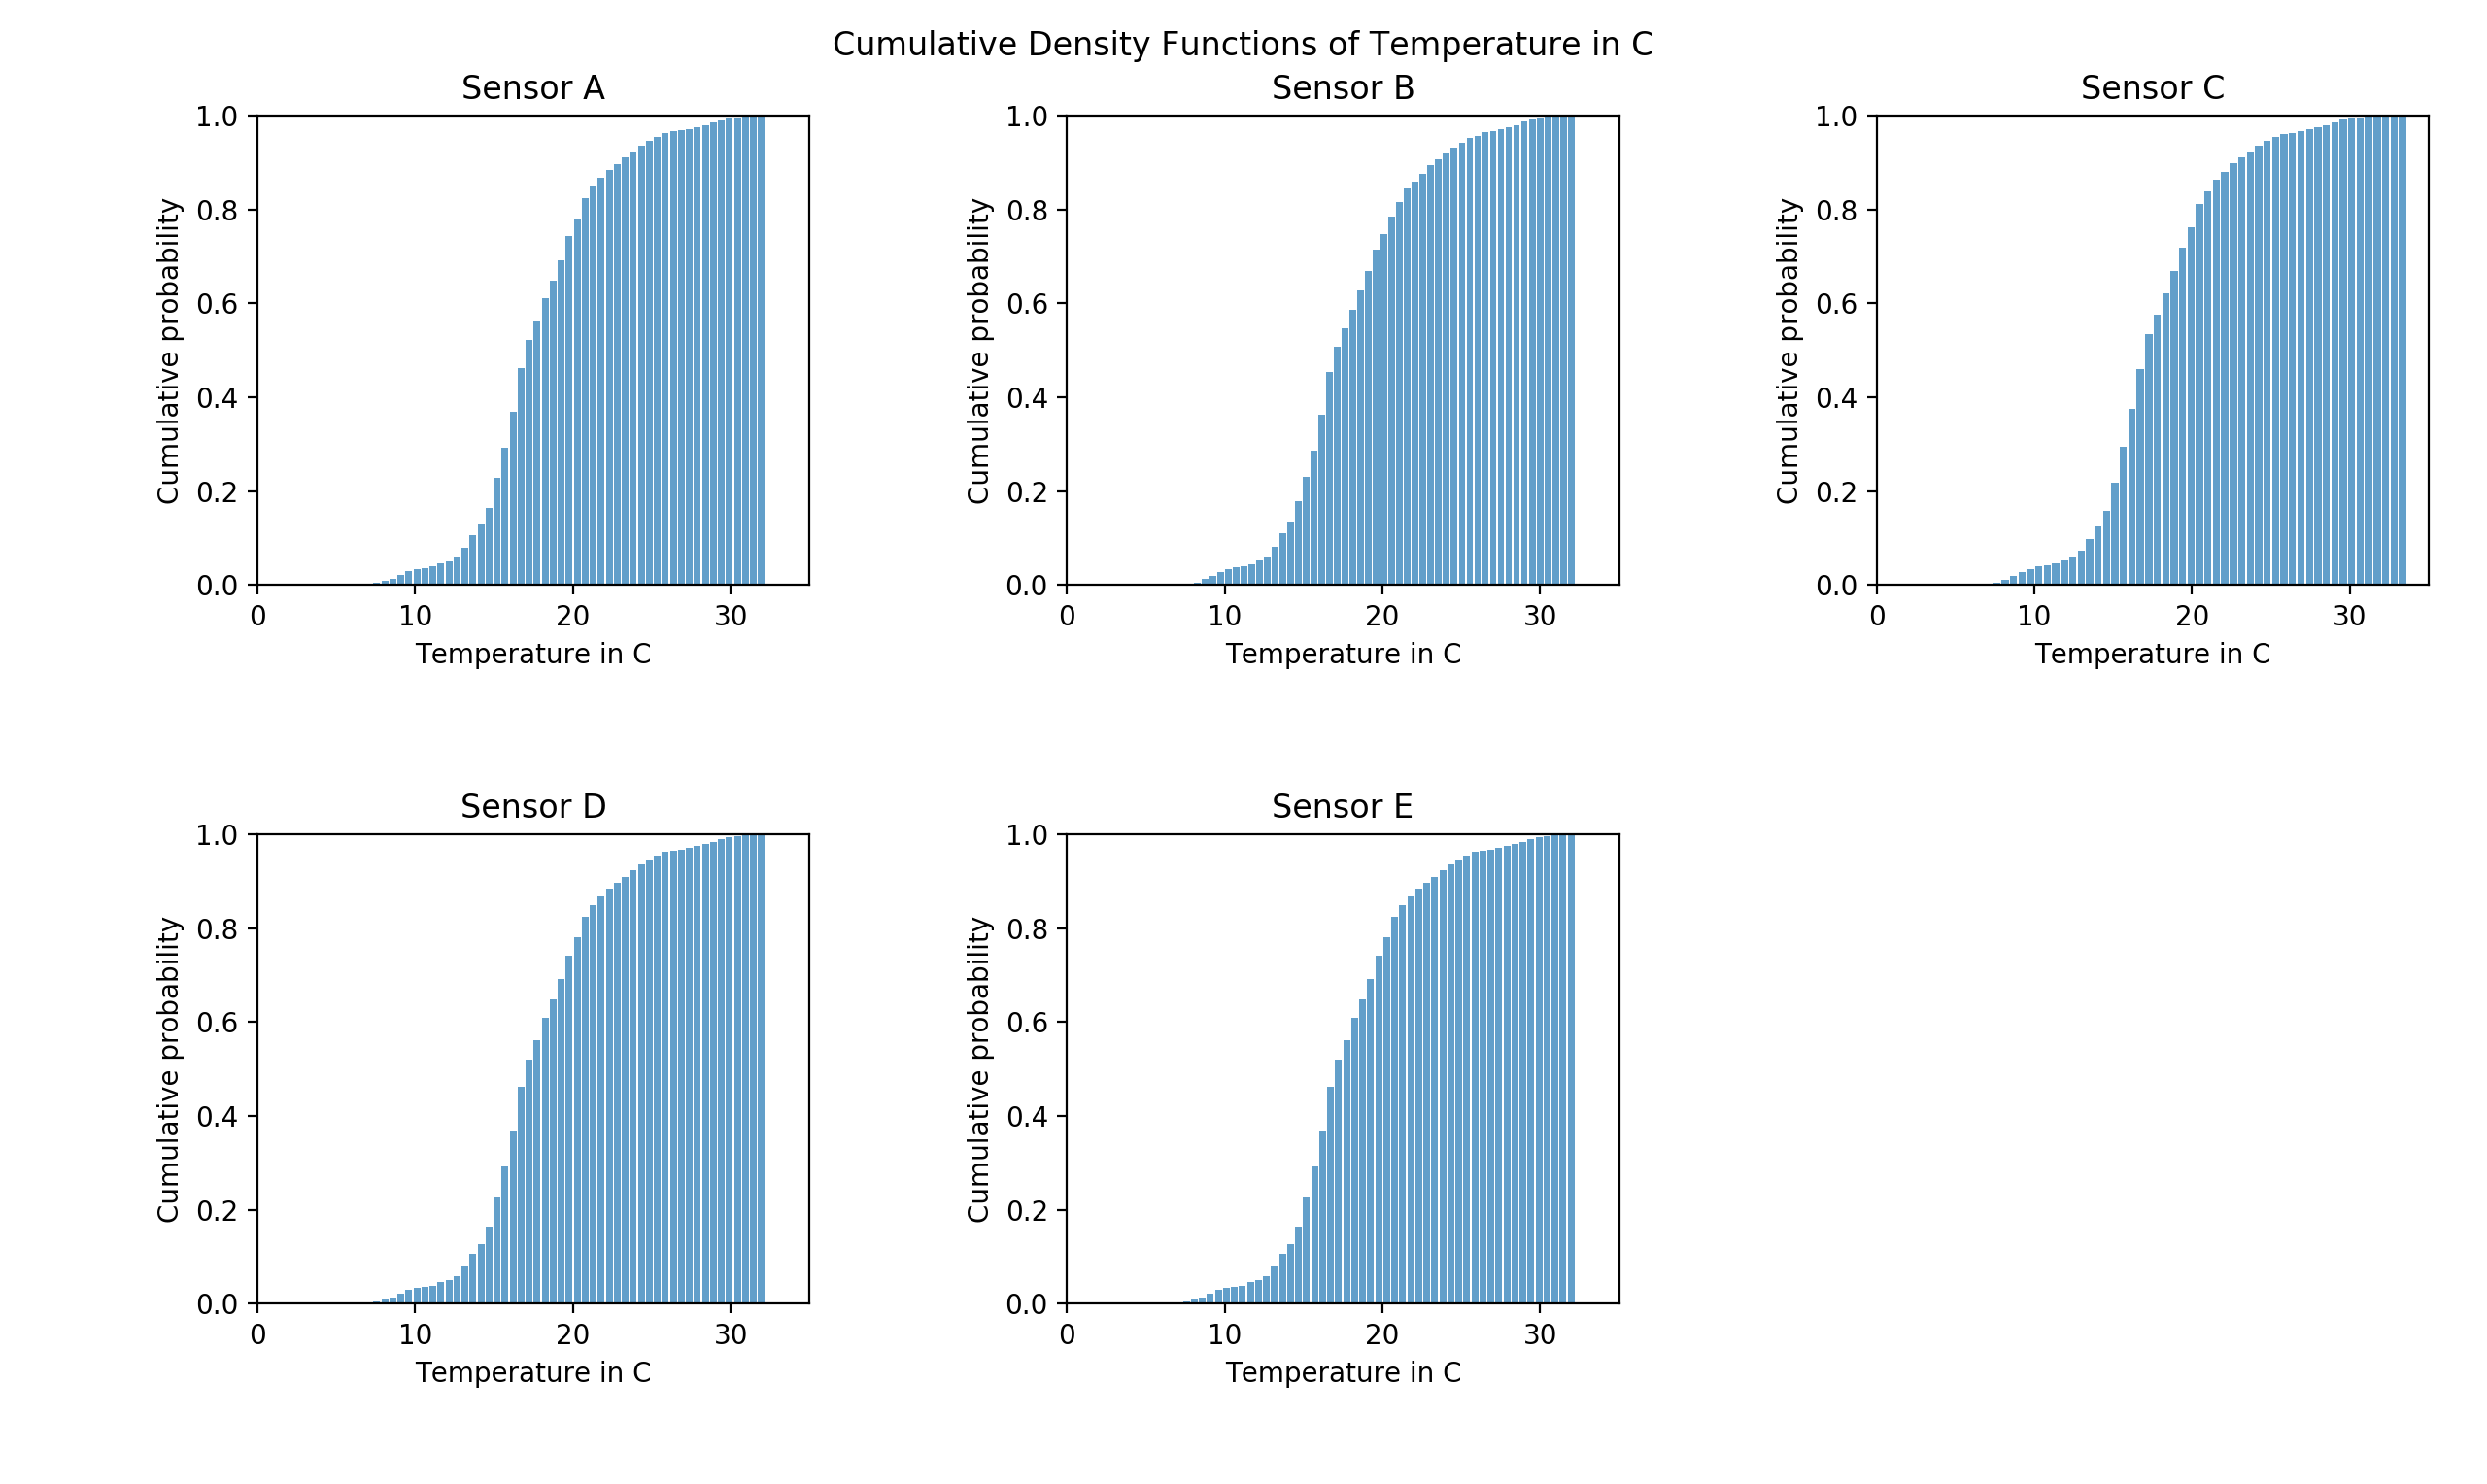
\includegraphics[width=\textwidth]{cdf_temp}
            \caption{Cumilative Density Functions of Temperature for all sensors}
        \end{figure}

        \begin{figure}[H]
            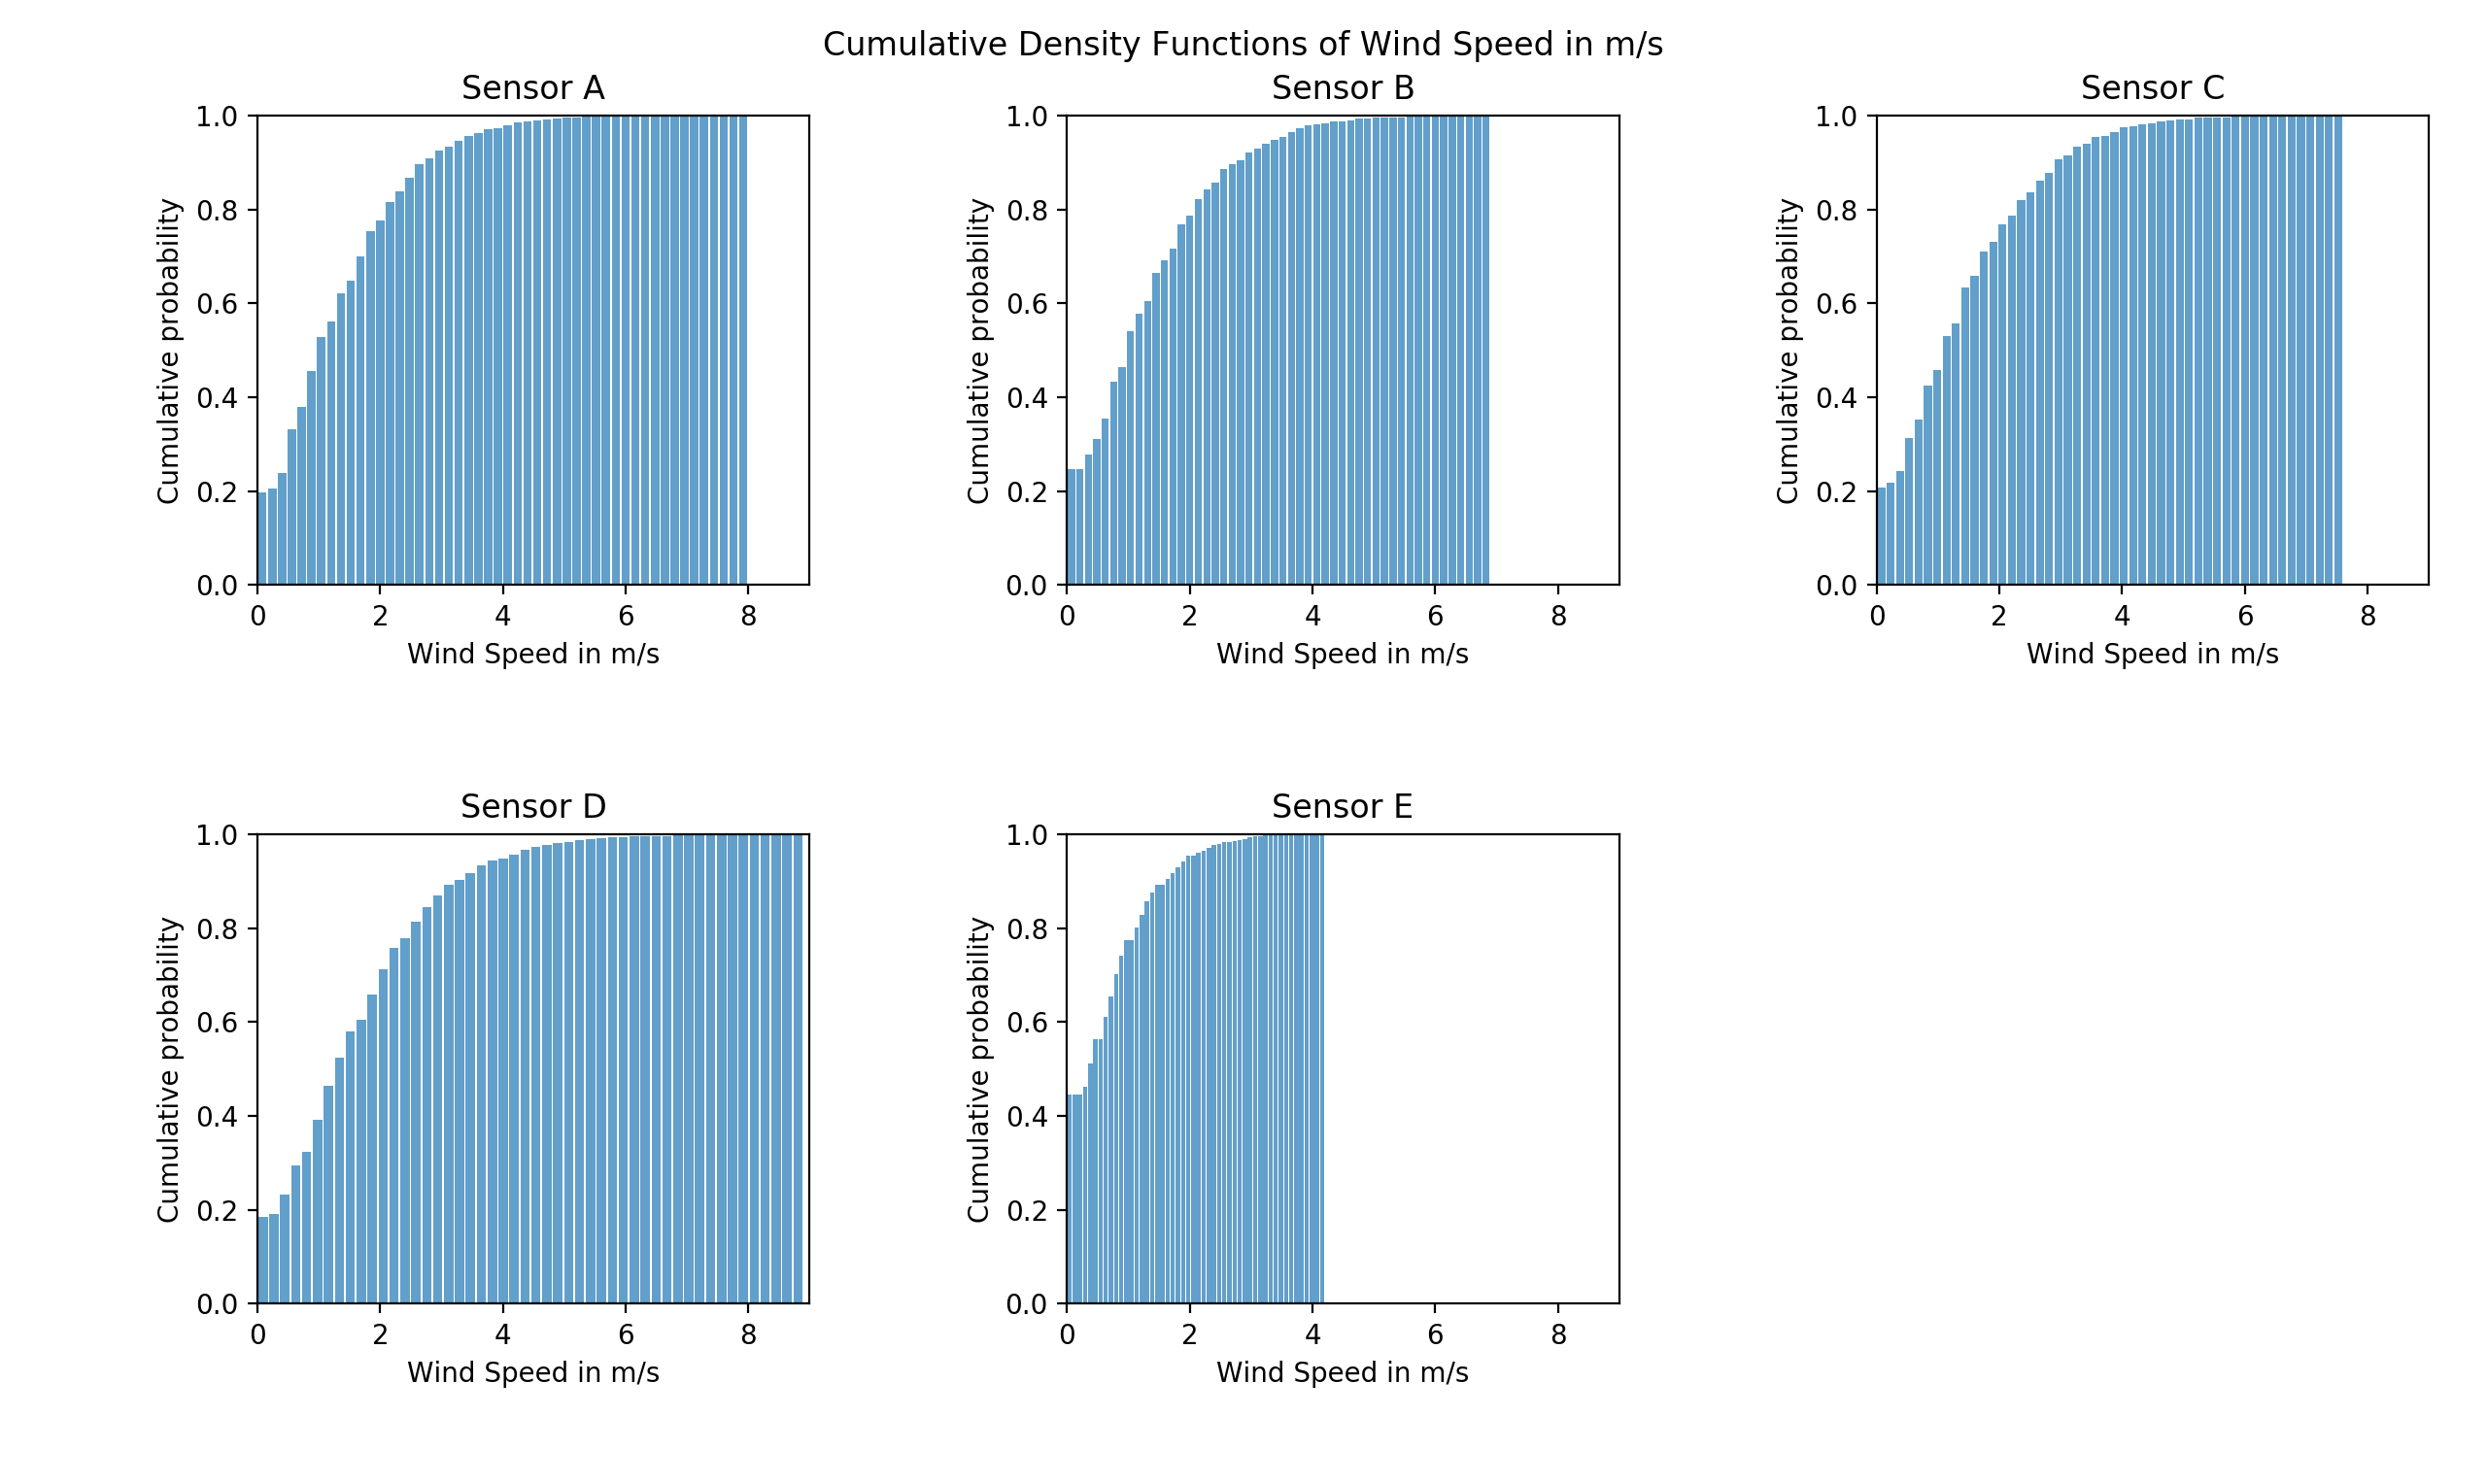
\includegraphics[width=\textwidth]{cdf_windspeed}
            \caption{Cumilative Density Functions of Wind Speed for all sensors}
        \end{figure}

    \subsection{Confidence Intervals}
        \begin{table}[H]
            \caption {Confidence intervals of Temperature for all sensors}
            \begin{tabular}{ll}
            & Temperature                              \\ \hline
            A & (17.81214113267346, 18.126065652463858)  \\
            B & (17.90472689963894, 18.226129320070267)  \\
            C & (17.754926235060246, 18.071347006653575) \\
            D & (17.83814660824381, 18.15457772482005)   \\
            E & (18.181933946027776, 18.525944841851015)
            \end{tabular}
            \end{table}

        \begin{table}[H]
            \caption {Confidence intervals of Wind Speed for all sensors}
            \begin{tabular}{ll}
            & Wind Speed                               \\ \hline
            A & (1.246227038990971, 1.3343868543854427)  \\
            B & (1.1971663346979249, 1.287082453670411)  \\
            C & (1.3243037885948932, 1.418622646328308)  \\
            D & (1.5296480419653757, 1.633650260379006)  \\
            E & (0.5680599051948441, 0.6244249432900044)
            \end{tabular}
            \end{table}

    \subsection{Hypothesis Test}
        \begin{table}[H]
            \caption {Confidence intervals of Wind Speed for all sensors}
            \begin{tabular}{lll}
                        & Temperature             & Wind Speed  \\ \hline
            p-value E, D & 0.0027270117155346967 & 4.899592405994867e-212  \\ 
            p-value C, D & 0.4657972008220813 & 4.610149126224334e-09  \\
            p-value B, C & 0.18562772895626528 & 9.40075204600199e-05  \\
            p-value A, B & 0.40185871871215073 & 0.13247973112544695 
            \end{tabular}
        \end{table}

        \ H0: $\mu 1$ = $\mu 2$ \ \\
        \ Ha: $\mu 2$ $\ne$ $\mu 2$ \\\
        The H0 is: the means of both sensors are the same. \\
        The Ha is: the means of the sensors are not the same. \\ \\
        For the Temperature variable, only the pair ED has a p-value below 0.05, which rejects 
        the null-hypothesis that the sensors are similar. All the other pairs have a p-value above
        the $\alpha$ of 0.05, so they are assumed to be similar. 
        \par For the variable Wind Speed pairs ED, CD and BC have a very low p-value, so the H0
        is rejected and they are not assumed similar. So, only pair AB is assumed similar for Wind Speed.

    \bibliographystyle{plain}
    \bibliography{references.bib}   

\end{document}